\documentclass[12pt,a4paper]{report}
\usepackage{tabularx}
\usepackage{array}
\usepackage{makecell}
\usepackage{listings}
\usepackage{styles/dolgozat}
\usepackage{svg}
\usepackage{graphicx}
\usepackage{styles/cpp}
\usepackage{styles/python}

\usepackage{hyperref}

% ── Globális listings beállítás (tördelés + magyar ékezetek) ─────────────────
\lstset{
  basicstyle=\small\ttfamily,
  breaklines=true,
  breakatwhitespace=false,
  breakindent=0pt,
  postbreak=\mbox{\textcolor{gray}{$\hookrightarrow$}\space},
  columns=flexible,
  keepspaces=true,
  showstringspaces=false,
  frame=single,
  frameround=tttt,
  backgroundcolor=\color[rgb]{0.95,0.95,0.95},
  rulecolor=\color[rgb]{0.85,0.85,0.85},
  framesep=6pt,
  xleftmargin=6pt,
  xrightmargin=6pt,
  literate=
    {á}{{\'{a}}}1 {é}{{\'{e}}}1 {í}{{\'\i}}1 {ó}{{\'{o}}}1
    {ö}{{\"o}}1  {ő}{{\H{o}}}1  {ú}{{\'{u}}}1 {ü}{{\"u}}1
    {ű}{{\H{u}}}1
    {Á}{{\'{A}}}1 {É}{{\'{E}}}1 {Í}{{\'{I}}}1 {Ó}{{\'{O}}}1
    {Ö}{{\"O}}1  {Ő}{{\H{O}}}1  {Ú}{{\'{U}}}1 {Ü}{{\"U}}1
    {Ű}{{\H{U}}}1,
}

\begin{document}

\include{cover/cimlap}

\newpage

\pagestyle{empty}

\include{cover/feladatkiiras}

\cleardoublepage
\pagenumbering{gobble}
\tableofcontents
\cleardoublepage
\pagenumbering{arabic}

\newpage

\pagestyle{fancy}

\include{chapters/1_introduction}
% új oszloptípus a tördeléshez
\newcolumntype{Y}{>{\raggedright\arraybackslash}X}


\Chapter{Koncepció}

\Section{Tartalom és felépítés}

Ebben a fejezetben a dolgozat témáját körülhatároljuk, bemutatjuk a releváns projektmenedzsment rendszereket, azok főbb funkcióit, előnyeit és hátrányait, valamint azt, hogyan kapcsolódnak az Acxor fejlesztéséhez. A cél nem a saját eredmények részletezése, hanem egy átfogó, irodalmi és technológiai alap bemutatása, amelyre a dolgozat további részei építenek. A fejezet négy fő területre koncentrál: irodalomkutatás, technológia, piackutatás és követelmény-specifikáció. Az irodalomkutatás során áttekintjük a legfontosabb projektmenedzsment rendszereket, a technológiai részben bemutatjuk a rendszerek főbb funkcióit, a piackutatás során összehasonlítjuk a meglévő megoldásokat, míg a követelmény-specifikációban az Acxor fejlesztés céljait és alapelveit foglaljuk össze.

\Section{Projektmenedzsment rendszerek áttekintése}

\SubSection{JIRA}

A JIRA egy komplex, vállalati szintű projektmenedzsment és issue tracking rendszer. Kiemelt jellemzői \cite{jira}:

\begin{itemize}
\item issue tracking, Agile metodikák (Scrum / Kanban) támogatása,
\item workflow testreszabás,
\item jogosultságkezelés,
\item riportok és dashboardok,
\item széleskörű integrációk (Confluence, Bitbucket, GitHub, Slack, Teams).
\end{itemize}

A JIRA rugalmas és szinte bármi testreszabható, ami előnyt jelent nagyvállalati környezetben, ugyanakkor komplexitása miatt tanulási görbéje meredek. A rendszer hierarchiája Epic–Story–Task–Subtask struktúrát követ, ami előnyös a nagy csapatok számára. Automatizmusai trigger–condition–action logikán alapulnak, amely lehetővé teszi például automatikus állapotváltást, assignee hozzárendelést, vagy e-mail értesítések küldését.

Az Acxor fejlesztésében a JIRA inspirációként szolgált a funkcionalitás és a workflow kezelés terén, de egyszerűsített felhasználói felületet és átláthatóbb jogosultsági modellt alkalmaz. A felület a \ref{fig:jira}. ábrán látható.

\begin{figure}[h!]
\centering
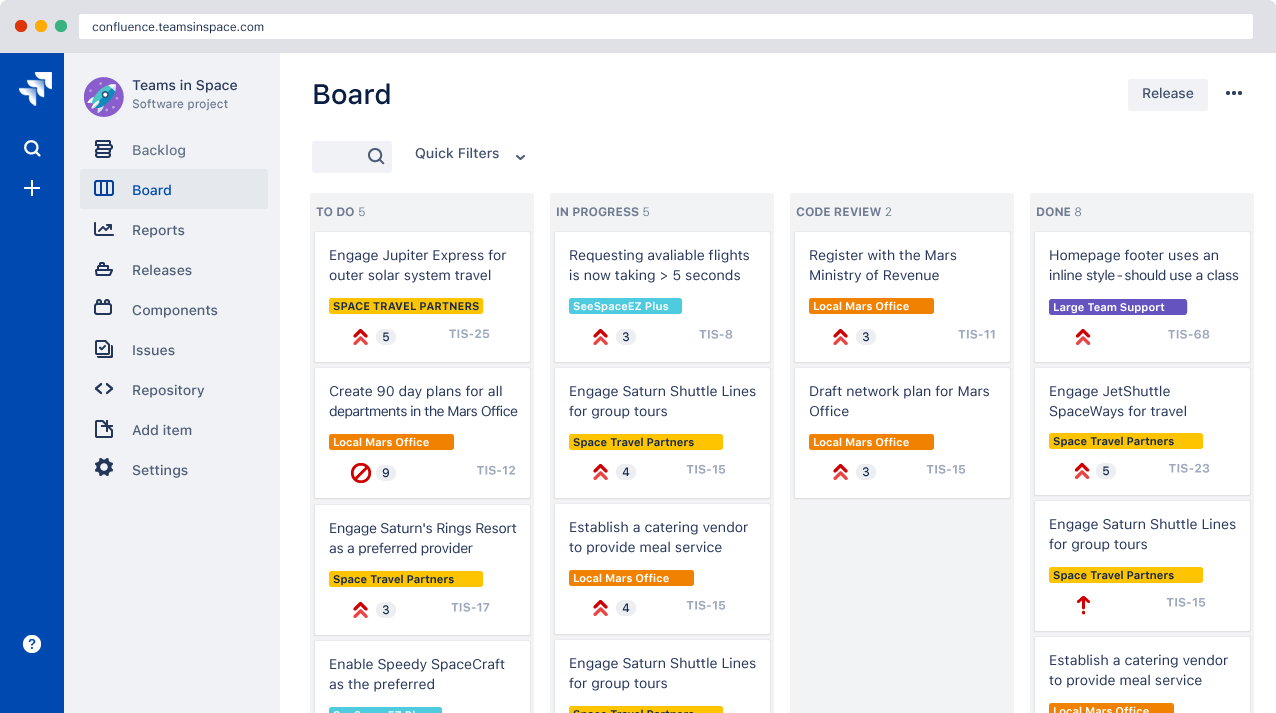
\includegraphics[width=0.75\textwidth]{images/jira.png}
\caption{A Jira sprint- és issue-kezelő felülete \cite{jira}}
\label{fig:jira}
\end{figure}

\SubSection{Trello}

A Trello egy intuitív, kártya-alapú projektmenedzsment rendszer, amely kisebb csapatoknak vagy egyszerűbb folyamatokhoz ideális. Főbb jellemzői \cite{trello}:

\begin{itemize}
\item Board → List → Card → Checklist vizuális hierarchia,
\item drag \& drop alapú kezelés,
\item minimális konfiguráció és real-time szinkron,
\item egyszerű automatizmusok (Butler).
\end{itemize}

A Trello előnye a gyors betanulás és a vizuális, átlátható felület, míg hátránya a korlátozott testreszabhatóság és a nagyobb projektekhez kevésbé megfelelő komplexitás. Az Acxor esetében a Trello inspirálta az intuitív, vizuális task lifecycle és board kezelést, amely egyszerre egyszerű és professzionális. A felület a \ref{fig:trello}. ábrán látható.

\begin{figure}[h!]
\centering
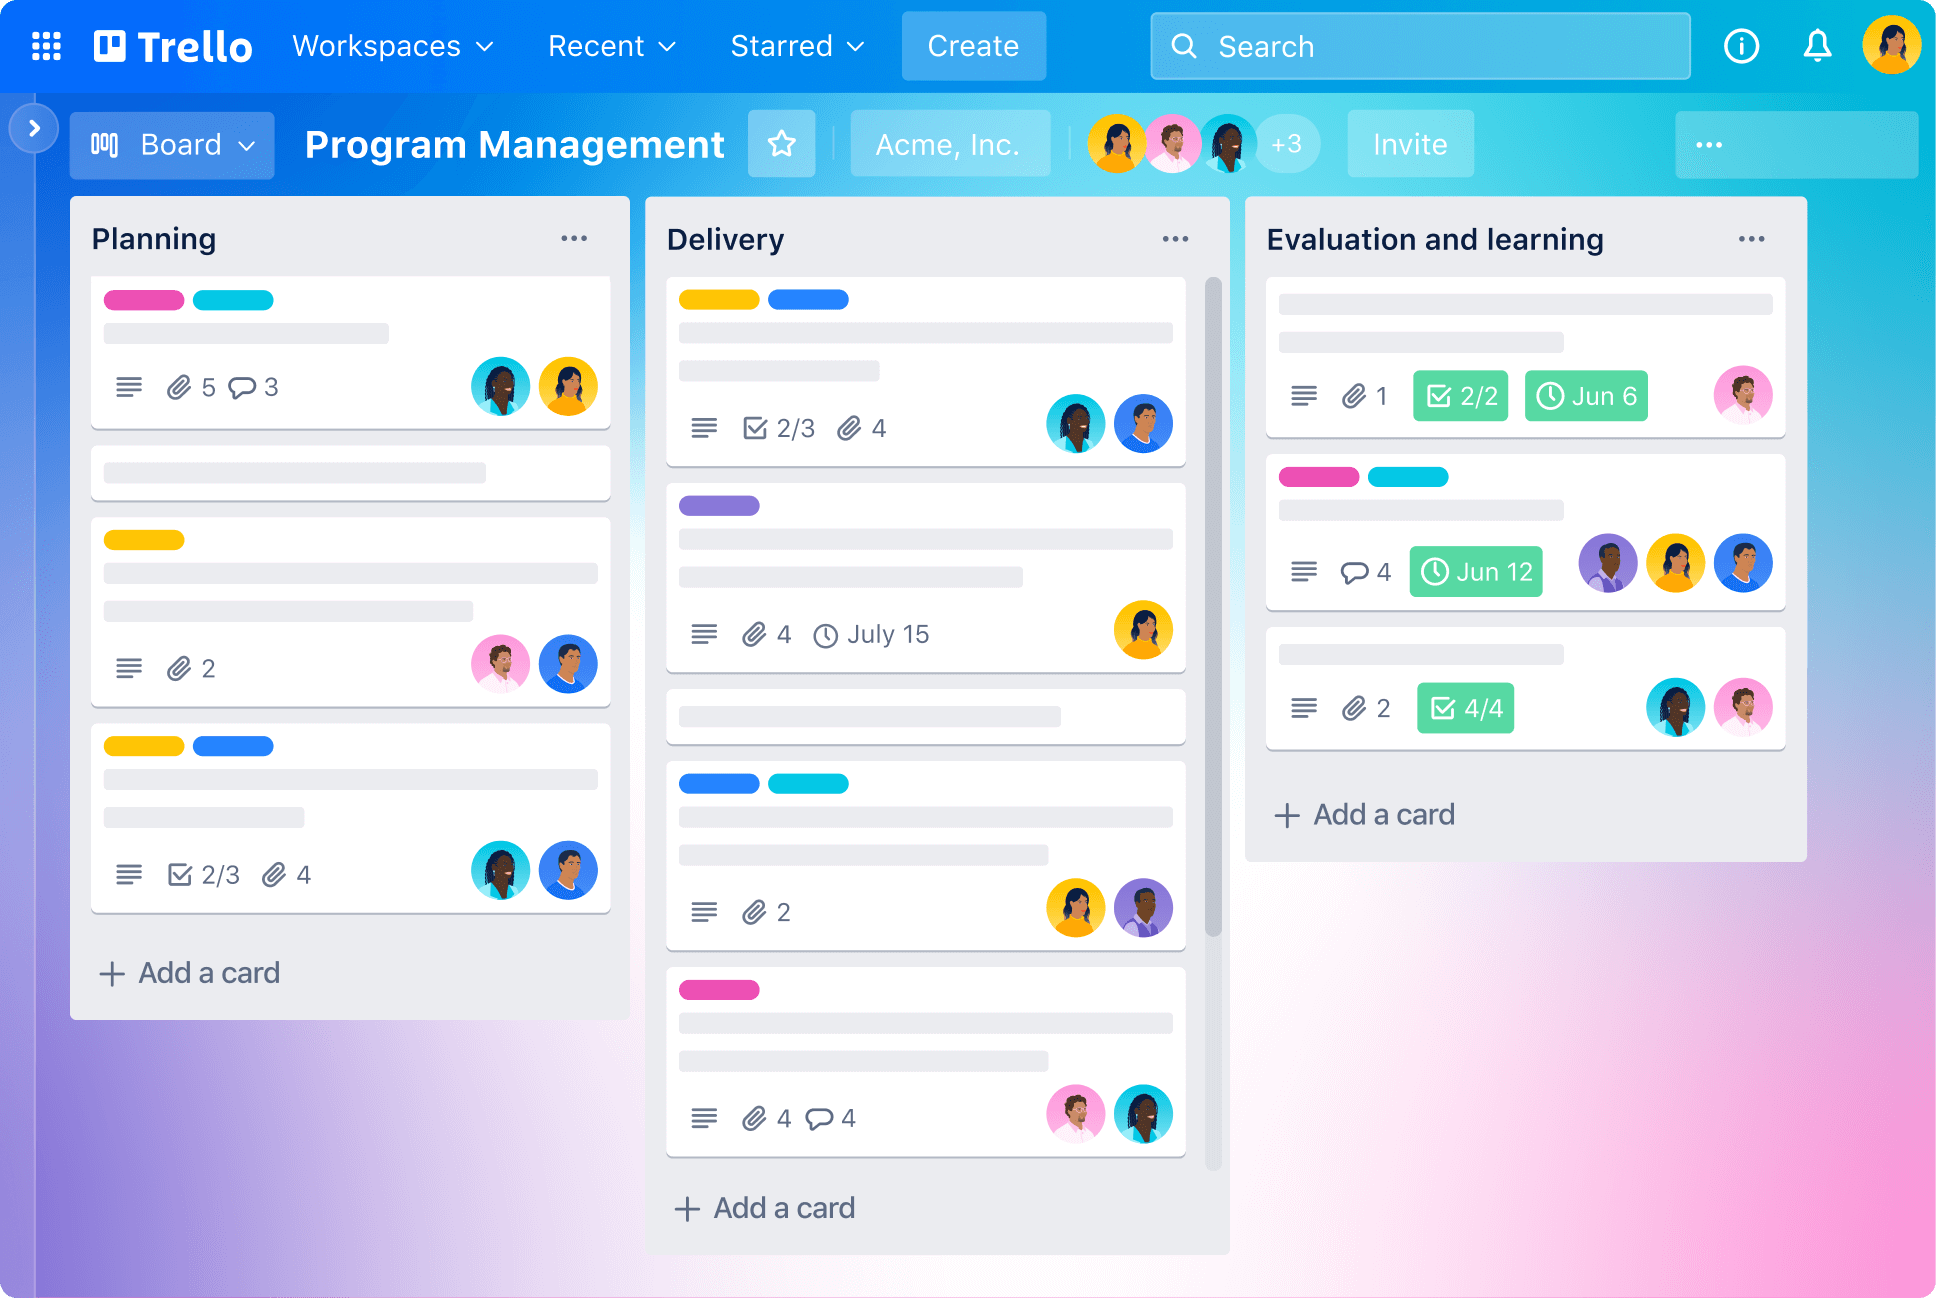
\includegraphics[width=0.8\textwidth]{images/trello.png}
\caption{A Trello Kanban-alapú feladatkezelő felülete \cite{trello}}
\label{fig:trello}
\end{figure}

\SubSection{Asana}

Az Asana egy feladat- és projektmenedzsment platform, amely a csapatok együttműködését támogatja. Fő funkciói \cite{asana}:

\begin{itemize}
\item task és subtask kezelés,
\item projektek és Timeline vizualizáció,
\item határidők és felelősök hozzárendelése,
\item dashboard és riporting,
\item integráció külső szolgáltatásokkal (Slack, Teams, GitHub, Google Workspace).
\end{itemize}

Előnye a könnyen átlátható felület és a gyors onboarding, hátránya a korlátozott workflow testreszabás és a részletes riporting hiánya. Az Acxor tervezésénél az Asana inspirációt jelentett a fókuszált task lifecycle és minimalista felület kialakításában. A felület a \ref{fig:asana}. ábrán látható.

\begin{figure}[h!]
\centering
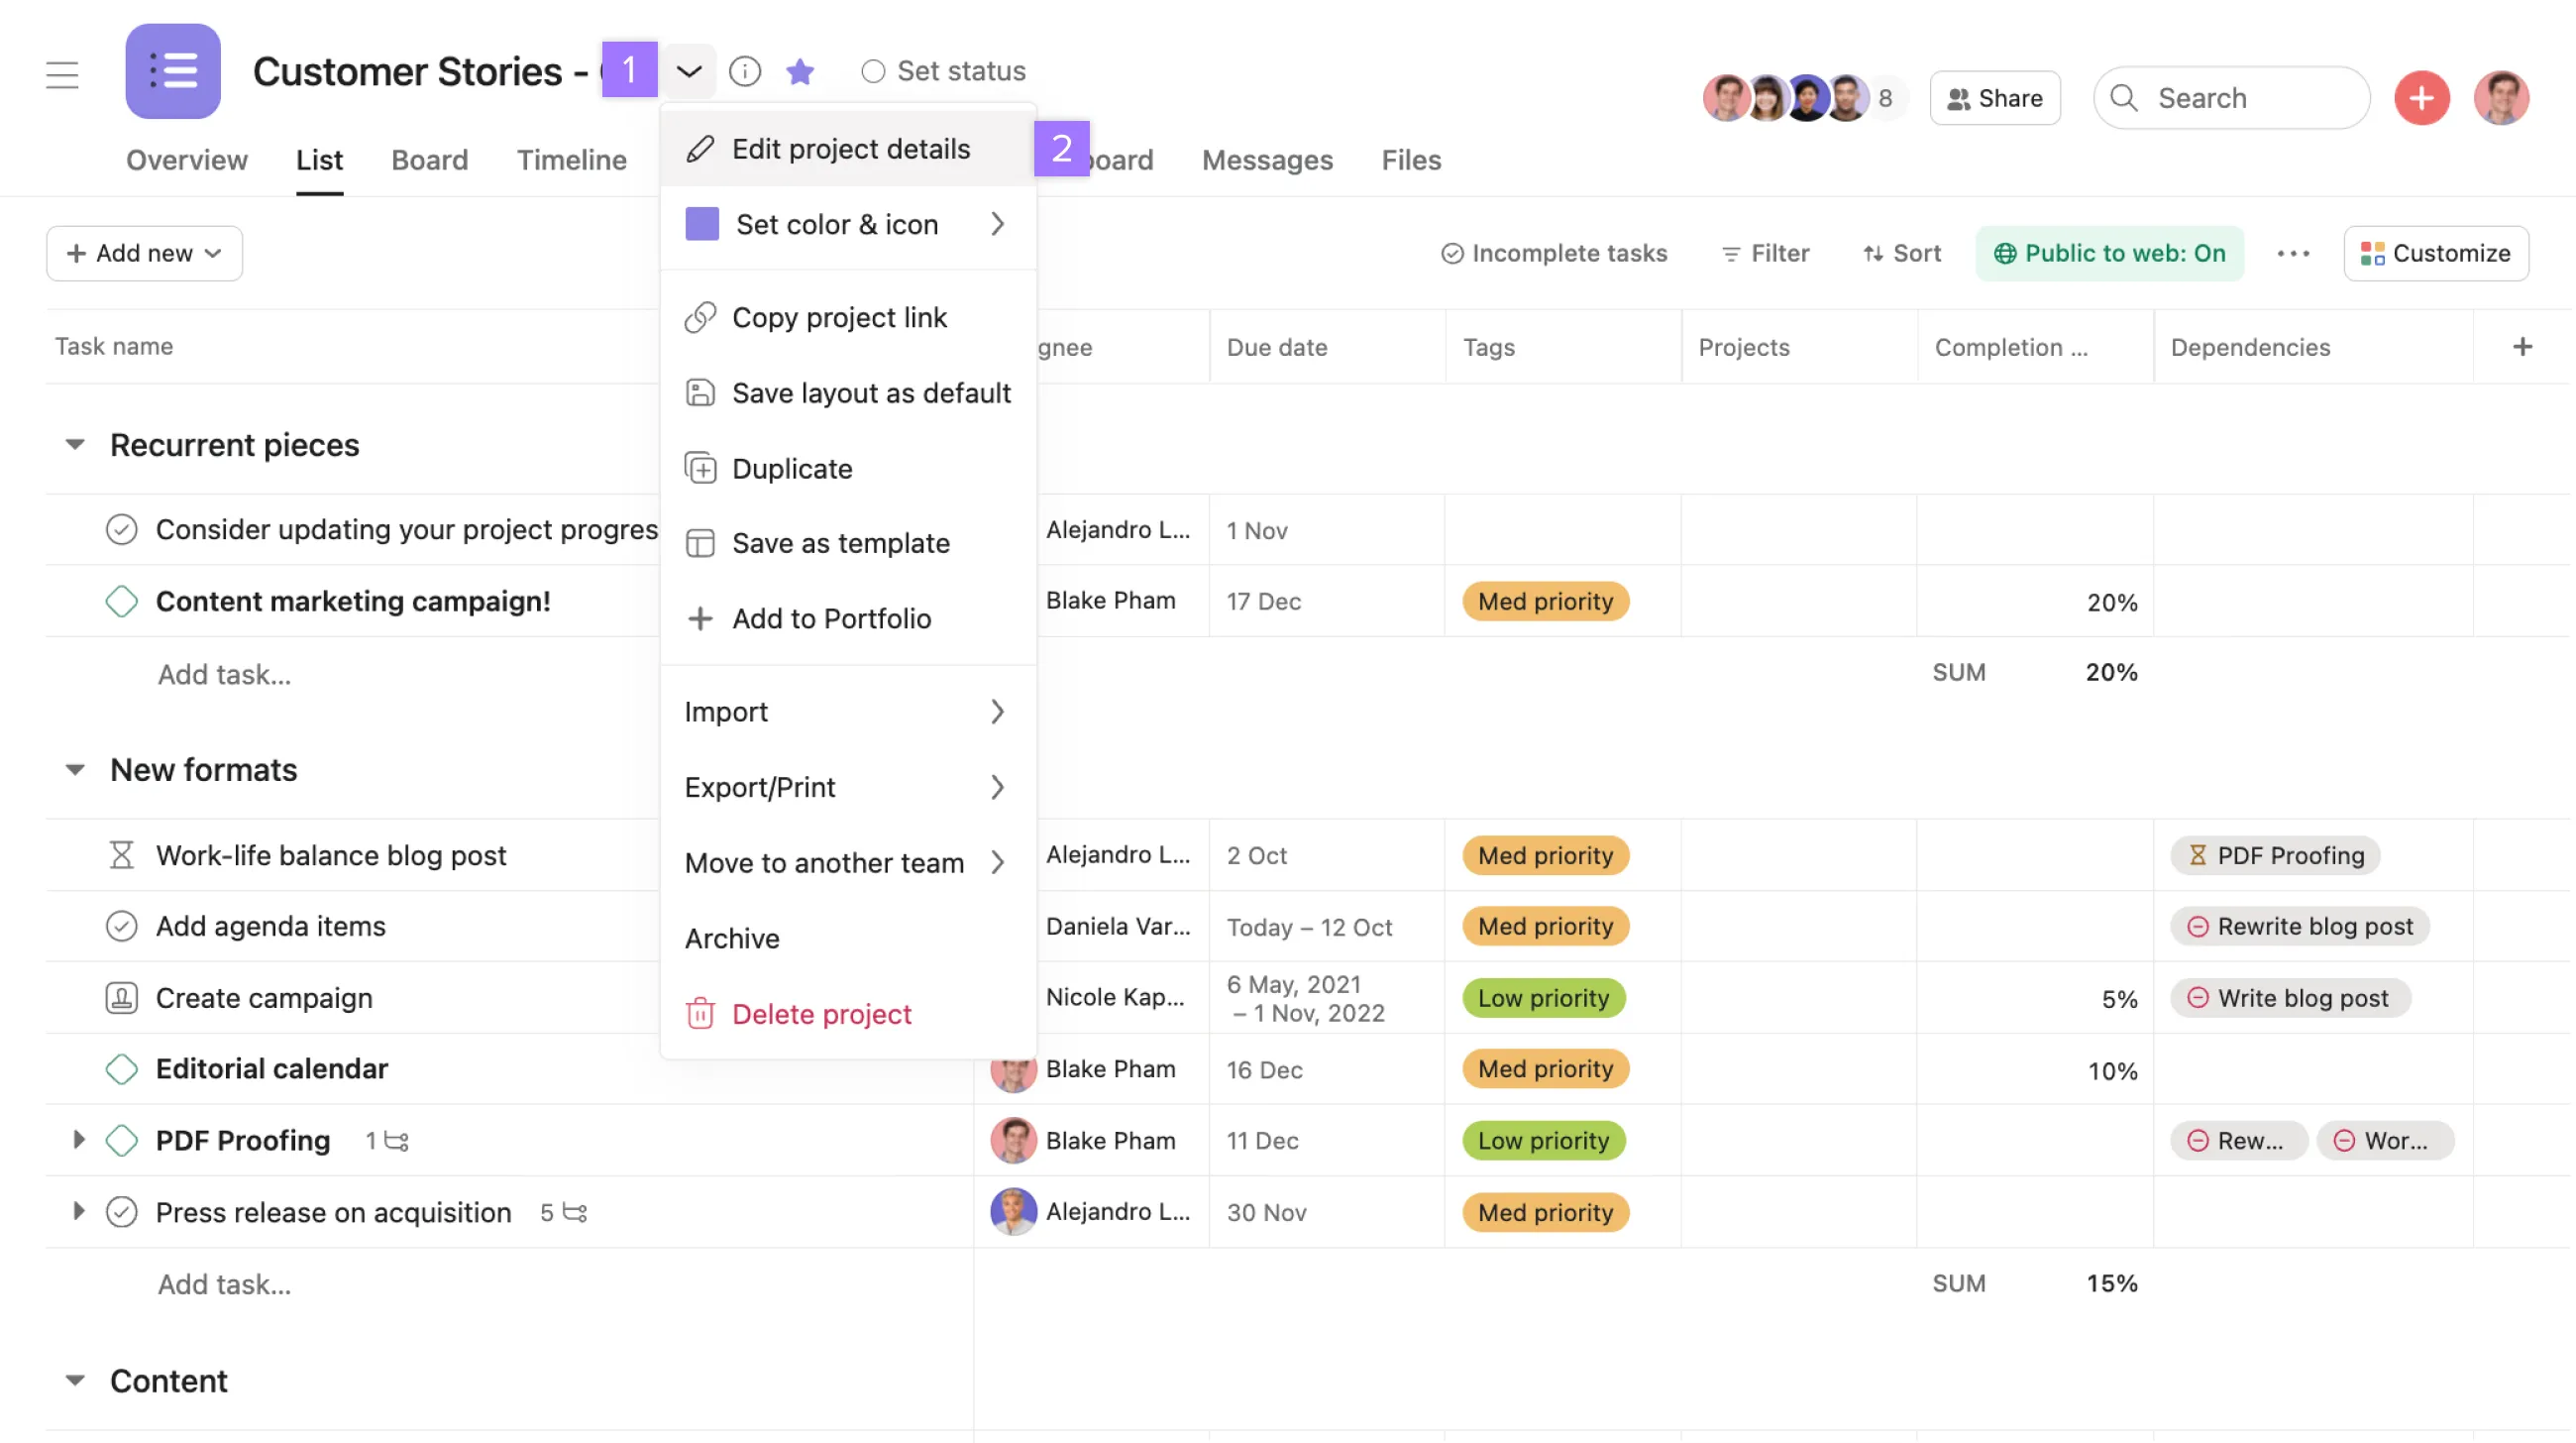
\includegraphics[width=0.8\textwidth]{images/asana.png}
\caption{Az Asana projektmenedzsment eszköz felülete \cite{asana}}
\label{fig:asana}
\end{figure}

\SubSection{Redmine}

A Redmine nyílt forráskódú rendszer, amely elsősorban testreszabhatóságáról és bővíthetőségéről ismert. Főbb jellemzői \cite{redmine}:

\begin{itemize}
\item issue tracking és projekt hierarchia (főprojekt → alprojekt),
\item testreszabható workflow és permission rendszer,
\item Gantt és Calendar vizualizáció,
\item plugin és API alapú integráció.
\end{itemize}

Előnye a nagy projektek kezelésére való alkalmasság és a nyílt forráskódú bővíthetőség, míg hátránya a kevésbé modern UI és a tanulási görbe. Az Acxorban a Redmine inspirációt jelentett a backend struktúrában és az issue hierarchia egyszerűsítésében, modern, letisztult felülettel. A felület a \ref{fig:redmine}. ábrán látható.

\begin{figure}[h!]
\centering
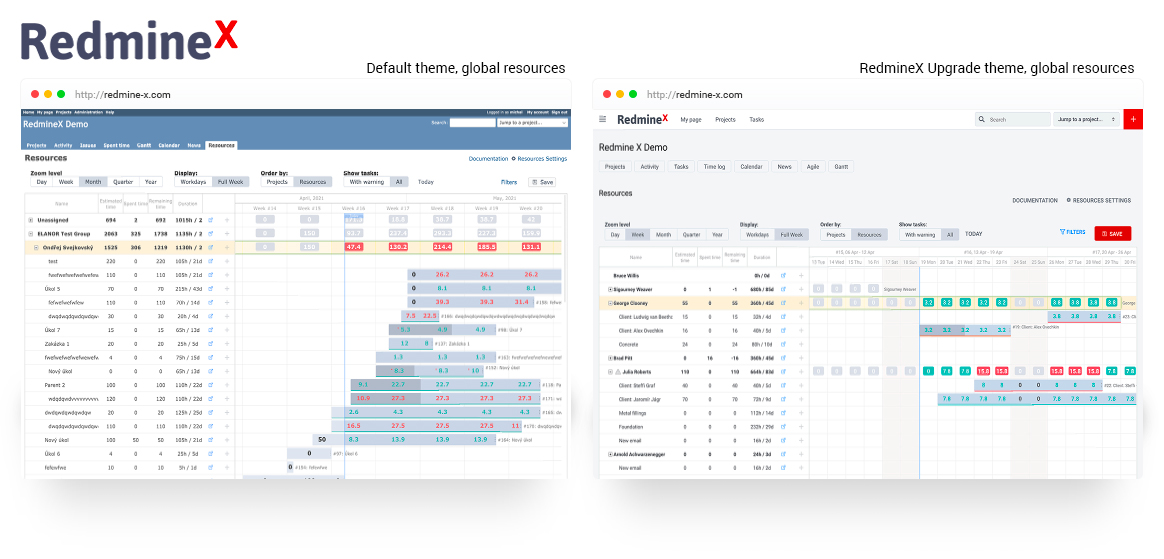
\includegraphics[width=0.8\textwidth]{images/redmine.jpg}
\caption{A Redmine nyílt forráskódú projektmenedzsment eszköz felülete \cite{redmine}}
\label{fig:redmine}
\end{figure}

\SubSection{Projektmenedzsment rendszerek összehasonlítása}

Az Acxor a közepes komplexitású fejlesztői csapatok számára készült, kiemelten figyelve a vizualitásra, egyszerűségre és motivációs rendszerekre. A \ref{tab:comparison1}. és \ref{tab:comparison2}. táblázat összehasonlítja az Acxort a Trello-val és a Jira-val, illetve a Redmine-nel és az Asana-val.

\begin{table}[h!]
\centering
\scriptsize
\setlength{\arrayrulewidth}{0.5pt}
\begin{tabularx}{\textwidth}{|l|Y|Y|Y|}
\hline
\textbf{Funkció / Eszköz} & \textbf{Acxor} & \textbf{Trello} & \textbf{Jira} \\
\hline
Webes felület & Modern vizuális UI & Webes, vizuális & Webes, komplex \\
Kanban board & Beépített, drag\&drop & Beépített & Részben, plugin szükséges \\
Sprint / Iteration & Részben, egyszerű & -- & Teljes körű \\
Gamifikáció & XP, szint, badge & -- & -- \\
Task / Subtask & \makecell[l]{Epic $\rightarrow$ Story \\ Task $\rightarrow$ Subtask} & Kártya / checklist & \makecell[l]{Epic $\rightarrow$ Story \\ Task $\rightarrow$ Subtask} \\
Chat / Log & Globális bot & Részben, kommentek & Részben, jegy alapú \\
Workflow testreszabás & Részben, egyszerű & Részben, limitált & Részletes, szabály alapú \\
Permission rendszer & Részben, egyszerű & Részben, egyszerű & Mély, szerepkör alapú \\
Integrációk & Alap, kulcs szolgáltatások & Részben, Power-Ups & Széles (Confluence, GitHub, Slack\ldots) \\
\hline
\end{tabularx}
\caption{Acxor összehasonlítása a Trello-val és a Jira-val \cite{trello, jira}}
\label{tab:comparison1}
\end{table}

\begin{table}[h!]
\centering
\scriptsize
\setlength{\arrayrulewidth}{0.5pt}
\begin{tabularx}{\textwidth}{|l|Y|Y|Y|}
\hline
\textbf{Funkció / Eszköz} & \textbf{Acxor} & \textbf{Redmine} & \textbf{Asana} \\
\hline
Webes felület & Modern vizuális UI & Webes, részletes & Webes, intuitív \\
Kanban board & Beépített & Részben, plugin szükséges & Board / list nézet \\
Sprint / Iteration & Részben, egyszerű & Teljes körű & Részben, idővonal / Timeline \\
Gamifikáció & XP, szint, badge & -- & -- \\
Task / Subtask & Egyszerű hierarchia & Issue / subtask & Task / subtask \\
Chat / Log & Globális bot & Részben, jegy alapú & Részben, kommentek \\
Workflow testreszabás & Részben, egyszerű & Részletes & Részben, egyszerű \\
Permission rendszer & Részben, egyszerű & Roles alapú & Részben, alap \\
Integrációk & Kulcs szolgáltatások & Részben, pluginok, SCM & Slack, GitHub, Google Workspace \\
\hline
\end{tabularx}
\caption{Acxor összehasonlítása a Redmine-nel és az Asana-val \cite{redmine, asana}}
\label{tab:comparison2}
\end{table}

A fenti rendszerek áttekintése rávilágít arra, hogy a projektmenedzsment eszközök széles skálán helyezkednek el komplexitás, testreszabhatóság és felhasználói élmény szempontjából. Az Acxor célja a különböző rendszerek előnyeinek ötvözése: a JIRA funkcionalitásának, a Trello vizuális egyszerűségének, az Asana átlátható task lifecycle-jának, valamint a Redmine struktúrájának kombinálása egy intuitív, könnyen használható, ugyanakkor professzionális projektmenedzsment platformban.

Ez a koncepciói alap biztosítja, hogy a dolgozat későbbi fejezeteiben bemutatott fejlesztések jól meghatározott, átgondolt irányelv szerint történjenek, és az olvasó számára érthető, követhető legyen a választott megközelítés és technológiai háttér.
\Chapter{Tervezés}

A tervezési fejezet célja az Acxor rendszer architektúrájának, adatmodelljének és felhasználói felületének részletes bemutatása. Ebben a fejezetben kerülnek ismertetésre azok a döntések, amelyek a fejlesztés irányvonalát meghatározták, beleértve a technológiai stack kiválasztását, az adatbázis-séma kialakítását, az API tervezését és a komponensstruktúrát. A tervezési fázis különösen fontos volt, hiszen a rendszernek három platformon – webes böngészőben, mobil eszközön és szerver oldalon – egyidejűleg kellett megfelelően működnie, miközben közös üzleti logikát és adatréteget használt.

% ─────────────────────────────────────────────────────────────────────────────
\Section{Rendszerarchitektúra}
% ─────────────────────────────────────────────────────────────────────────────

Az Acxor rendszer három jól elkülönülő részből áll: a webes frontend alkalmazásból, a React Native alapú mobil alkalmazásból és a Node.js backend API-ból. Mindhárom rész egyetlen közös RESTful API-on keresztül kommunikál, amelyet a backend szolgáltat. Ez a megközelítés lehetővé teszi, hogy a kliens oldalak teljesen független életet éljenek, miközben ugyanazokat az adatokat, autentikációs mechanizmust és üzleti szabályokat alkalmazzák. Az architektúra tehát klasszikus kliens-szerver modellt követ, azzal a kiegészítéssel, hogy két teljesen különböző típusú kliens is ugyanahhoz a backendhez csatlakozik.

\begin{figure}[h!]
\centering
% IDE KERÜL: Rendszerarchitektúra diagram (három réteg: Mobile App, Web App, Backend API + MongoDB)
\fbox{\parbox{12cm}{\centering\vspace{3cm} [Rendszerarchitektúra-diagram: Web (React/Vite) $\leftrightarrow$ REST API (Node.js/Express) $\leftrightarrow$ MongoDB, Mobile (React Native/Expo) $\leftrightarrow$ REST API] \vspace{3cm}}}
\caption{Az Acxor rendszer magas szintű architektúrája}
\label{fig:architecture}
\end{figure}

A backend alkalmazás Express.js keretrendszeren alapul, és a következő főbb feladatokat látja el: felhasználói hitelesítés (JWT), projektek, feladatok és alfeladatok kezelése, sprintek és napló bejegyzések tárolása, XP-alapú gamifikációs logika végrehajtása, valamint GitHub API-val való integráció. Az adatok MongoDB adatbázisban tárolódnak, amelyhez a Mongoose ODM biztosít séma-alapú hozzáférést.

A webes frontend Vite segítségével épített React alkalmazás, amely Tailwind CSS-t használ a stílusok kialakítására. Az állapotkezelés React Context API-n és \texttt{useReducer} hookson alapul, amelyek Redux-szerű, de külső könyvtártól független megoldást nyújtanak. A mobil alkalmazás Expo keretrendszerre épített React Native projekt, amely ugyanolyan üzleti logikát követ, mint a webes változat, azonban natív mobil UI komponenseket alkalmaz.

% ─────────────────────────────────────────────────────────────────────────────
\Section{Technológiai stack}
% ─────────────────────────────────────────────────────────────────────────────

A fejlesztés során a technológiai döntések több szempontot is figyelembe vettek: a fejlesztői ökoszisztéma érettségét, a közösségi támogatottságot, a típusbiztonságot, valamint azt, hogy a választott technológiák lehetővé tegyék a gyors prototípuskészítést anélkül, hogy a kód minőségét veszélyeztetnék.

\SubSection{Backend}

A backend Node.js és TypeScript kombinációjára épül. A TypeScript alkalmazása biztosítja a statikus típusellenőrzést, ami különösen hasznos az API végpontok bemeneti és kimeneti adatainak validálásakor. Az Express.js a defacto standard REST API keretrendszer Node.js alatt, amelynek middleware-alapú felépítése rugalmasan bővíthető. A MongoDB dokumentumorientált adatbázis jól illeszkedik a projektmenedzsment adatok természetéhez, ahol a rugalmas sémák lehetővé teszik a feladatok, alfeladatok és projektek összetett struktúráinak tárolását. A Mongoose ODM séma validációt és referencia-alapú kapcsolatokat biztosít a dokumentumok között.

A hitelesítés JSON Web Token alapon működik. Bejelentkezéskor a szerver egy 7 napos érvényességű tokent állít ki, amelyet a kliens minden API kéréshez csatol az \texttt{Authorization} fejlécben. A jelszavak bcryptjs segítségével kerülnek hashelésre, 10-es salt rounds értékkel. A védett végpontokat egy \texttt{protect} middleware védi, amely ellenőrzi a token érvényességét és azonosítja a felhasználót.

\SubSection{Webes frontend}

A webes alkalmazás React 18-ra épül, Vite fejlesztői szerverrel és build eszközzel. A Tailwind CSS utility-first megközelítése lehetővé tette a gyors és következetes stílusok kialakítását anélkül, hogy külön CSS fájlokat kellett volna karbantartani. Az állapotkezelés teljesen egyedi megoldást alkalmaz: a \texttt{GlobalContext} tárolja az alkalmazás fő adatait (felhasználó, projektek, feladatok, alfeladatok, sprintek), míg a \texttt{ViewContext} a nézetek közötti navigációért felelős. Az axios könyvtár HTTP kérések küldésére szolgál a webes kliensben.

\SubSection{Mobil frontend}

A mobil alkalmazás React Native alapú, Expo keretrendszerrel. Az Expo lehetővé teszi a gyors fejlesztést és az eszközön való tesztelést Expo Go segítségével. A navigáció Expo Router révén fájlrendszer-alapú, ami közelebb áll a Next.js szemléletéhez. A mobil alkalmazás a fetch API-t alkalmazza HTTP kérésekhez, és a backend ugyanazon végpontjait éri el, mint a webes kliens. Az állapotkezelés megegyezik a webes verzióéval: Context API és useReducer kombináció.

% ─────────────────────────────────────────────────────────────────────────────
\Section{Adatbázis-tervezés}
% ─────────────────────────────────────────────────────────────────────────────

Az adatbázis tervezésekor a legfontosabb szempontok a normalizált, de praktikusan használható séma kialakítása volt. A MongoDB dokumentumorientált természete lehetővé tette a referencia-alapú kapcsolatok (ObjectId hivatkozások) és a beágyazott dokumentumok vegyítését. A rendszer összesen hét Mongoose modellt alkalmaz.

\SubSection{Adatmodellek}

A \texttt{User} modell tartalmazza a felhasználói adatokat, köztük a gamifikációhoz szükséges \texttt{xp}, \texttt{level} és \texttt{prestige} mezőket. A \texttt{Project} dokumentum tárolja az adminisztrátor, a közreműködők és a megtekintők referenciáit, ezáltal biztosítva az alapszintű hozzáférésvezérlést. A \texttt{Task} modell egy projektre és opcionálisan egy sprintre mutat, emellett tartalmaz \texttt{xpReward}, \texttt{deadline} és \texttt{assignedTo} mezőket. A \texttt{Subtask} modell szülő feladathoz kapcsolódik, és hasonló szerkezetet követ. A \texttt{Sprint} modell projekthez tartozik, és dátumtartománnyal rendelkezik. A \texttt{Log} modell eseménynaplózásra szolgál, projekt-szinten. A \texttt{Mail} modell a felhasználók közötti üzenetküldést teszi lehetővé.

\begin{figure}[h!]
\centering
% IDE KERÜL: ER diagram (Entity-Relationship) az összes modellel és kapcsolataikkal
% User -- Project (admin, contributors, viewers, members)
% Project -- Task (project ref)
% Task -- Subtask (task ref)
% Project -- Sprint (project ref)
% Task -- Sprint (sprint ref, opcionális)
% Project -- Log (project ref)
% User -- Log (user ref, opcionális)
% User -- Mail (from, to ref)
\fbox{\parbox{14cm}{\centering\vspace{5cm} [ER-diagram: User, Project, Task, Subtask, Sprint, Log, Mail entitások és kapcsolataik (ObjectId referenciák jelölve)] \vspace{5cm}}}
\caption{Az Acxor adatbázis-séma ER-diagramja}
\label{fig:er-diagram}
\end{figure}

Az alábbi táblázat összefoglalja a főbb modellek legfontosabb mezőit:

\begin{table}[h!]
\centering
\small
\begin{tabularx}{\textwidth}{|l|l|Y|}
\hline
\textbf{Modell} & \textbf{Mező} & \textbf{Leírás} \\
\hline
User & username, email, password & Alapadatok, egyedi azonosítók \\
     & xp, level, prestige & Gamifikációs állapot \\
     & role, verified, avatar & Jogosultság és profil \\
\hline
Project & name, description & Projekt azonosítása \\
        & admin, contributors, viewers, members & Hozzáférésvezérlés (ObjectId ref.) \\
        & createdBy & Tulajdonos \\
\hline
Task & title, status & Feladat neve és állapota \\
     & project, sprint & Szülő referenciák \\
     & assignedTo, deadline, xpReward & Hozzárendelés és jutalom \\
\hline
Subtask & title, status & Alfeladat neve és állapota \\
        & task, assignedTo, xpReward & Szülő feladat és jutalom \\
\hline
Sprint & name, project, startDate, endDate & Sprint adatok \\
\hline
Log & project, message, user & Naplóbejegyzés \\
\hline
Mail & from, to, subject, body, read & Üzenet adatok \\
\hline
\end{tabularx}
\caption{Az adatmodellek főbb mezői}
\label{tab:models}
\end{table}

\SubSection{XP és szintlépési rendszer tervezése}

A gamifikációs rendszer tervezésekor fontos szempont volt, hogy a szintlépési formula megfelelően skálázódjon: az alacsonyabb szinteken legyen könnyen teljesíthető, de magasabb szinteken és presztízs értéknél egyre több munkát igényeljen. A választott formula:

\begin{equation}
\text{XP szükséges} = 20 + (\text{következő szint} \times 10) + (\text{prestige} \times \text{szint} \times 10)
\label{eq:xp-formula}
\end{equation}

Ez a formula biztosítja, hogy az első szintlépés viszonylag kevés XP-vel elérhető, ugyanakkor a prestige rendszer exponálisan növeli a szintenként szükséges XP mennyiséget. Az \texttt{addXP} service függvény a szintlépési logikát egy \texttt{while} ciklusban kezeli, hogy egyszerre több szinten is lehetséges legyen lépni, ha elég XP gyűlik össze. A jutalmak a következők: befejezett feladat esetén alapértelmezetten 5 XP, befejezett alfeladat esetén 3 XP jár a felelős felhasználónak.

% ─────────────────────────────────────────────────────────────────────────────
\Section{API tervezés}
% ─────────────────────────────────────────────────────────────────────────────

Az API RESTful elveket követ: az erőforrások azonosítása URL-eken keresztül történik, az HTTP metódusok (GET, POST, PUT, DELETE) jelölik a szándékot, a válaszok JSON formátumúak, és a megfelelő HTTP státuszkódok kerülnek visszaadásra. Az összes érzékeny végponthoz Bearer token alapú hitelesítés szükséges.

\SubSection{Végpont-struktúra}

Az API végpontjai a következő fő útvonalcsoportokra oszthatók:

\begin{itemize}
\item \texttt{/api/auth} -- Regisztráció és bejelentkezés
\item \texttt{/api/projects} -- Projektek CRUD műveletek
\item \texttt{/api/tasks} -- Feladatok kezelése, befejezés XP-vel
\item \texttt{/api/subtasks} -- Alfeladatok kezelése, befejezés XP-vel
\item \texttt{/api/sprints} -- Sprintek és feladat hozzárendelés
\item \texttt{/api/logs} -- Projektek aktivitásnaplója
\item \texttt{/api/users} -- Saját profil lekérése és módosítása
\item \texttt{/api/mails} -- Belső üzenetrendszer
\item \texttt{/api/github} -- GitHub integrációs végpontok
\end{itemize}

\begin{figure}[h!]
\centering
% IDE KERÜL: Swagger UI képernyőkép a főbb API végpontokkal
% (pl. a /api/tasks, /api/projects, /api/auth végpontok listája a Swagger dokumentációban)
\fbox{\parbox{14cm}{\centering\vspace{4cm} [Swagger UI képernyőkép: az API végpontok listája csoportosítva (auth, projects, tasks, subtasks, sprints, logs, users, mails, github)] \vspace{4cm}}}
\caption{Az Acxor REST API dokumentációja (Swagger UI)}
\label{fig:swagger}
\end{figure}

\SubSection{Hitelesítési folyamat}

A hitelesítés kétlépéses folyamat: regisztrációkor a szerver bcrypt segítségével hasheli a jelszót, majd JWT tokent állít ki. Bejelentkezéskor az elküldött jelszót összehasonlítja a tárolt hashsel, és sikeres egyezés esetén új tokent bocsát ki. A token tartalmazza a felhasználó azonosítóját (\texttt{id} mező), 7 napos érvényességgel. A védett middleware a tokent dekódolja, megkeresi az adatbázisban a felhasználót, és ha megtalálja, csatolja a \texttt{req.user} objektumhoz a további feldolgozáshoz.

\begin{figure}[h!]
\centering
% IDE KERÜL: Szekvenciadiagram a bejelentkezési folyamatról
% Client -> POST /api/auth/login -> Server -> bcrypt.compare -> JWT sign -> Client (token)
% Következő kérés: Client -> Bearer token -> protect middleware -> User lookup -> Controller
\fbox{\parbox{12cm}{\centering\vspace{3.5cm} [Szekvenciadiagram: bejelentkezési és hitelesítési folyamat (JWT kiállítás és validálás)] \vspace{3.5cm}}}
\caption{A JWT alapú hitelesítési folyamat szekvenciadiagramja}
\label{fig:auth-sequence}
\end{figure}

\SubSection{Feladat-befejezési folyamat}

A feladatok befejezése nem az általános UPDATE végponton keresztül történik, hanem egy dedikált \texttt{PUT /api/tasks/:id/complete} végponton. Ez a döntés azért született, mert a befejezéshez kapcsolódó logika (XP jóváírás, naplóbejegyzés írása) komplex mellékhatásokat von maga után, amelyeket el kell különíteni az egyszerű adatmódosítástól. A befejezési végpont ellenőrzi, hogy a feladat korábban már el volt-e végezve (\texttt{alreadyDone} jelző), és csak az első befejezéskor ír jóvá XP-t. Hasonló logika érvényes az alfeladatokra is.

% ─────────────────────────────────────────────────────────────────────────────
\Section{Use case tervezés}
% ─────────────────────────────────────────────────────────────────────────────

A rendszer főbb használati esetei a következő szereplők köré szerveződnek: vendég felhasználó (nem bejelentkezett), alapfelhasználó (bejelentkezett), és projekt adminisztrátor (a projekt létrehozója). A vendég felhasználók csak a főoldalt és a wiki oldalt tekinthetik meg. Az alapfelhasználók projekteket hozhatnak létre és kezelhetnek, feladatokat adhatnak hozzá és zárhatnak le, belső üzeneteket küldhetnek, és követhetik a gamifikációs előrehaladásukat. A projekt adminisztrátor emellett módosíthatja és törölheti a projektet, és kezelheti a közreműködők listáját.

\begin{figure}[h!]
\centering
% IDE KERÜL: Use case diagram (UML)
% Actors: Vendég, Felhasználó, Projekt Admin
% Use cases: Regisztráció, Bejelentkezés, Projekt létrehozás (GitHub / kézi),
%            Feladat hozzáadás, Feladat szerkesztés/törlés, Alfeladat kezelés,
%            Sprint kezelés, Kanban megtekintés, Plan megtekintés,
%            Gamifikáció megtekintés, Mail küldés, Log megtekintés,
%            Profil szerkesztés, Projekt törlés
\fbox{\parbox{14cm}{\centering\vspace{5cm} [UML Use Case diagram: Vendég, Felhasználó, Projekt Admin szerepkörök és a hozzájuk tartozó használati esetek] \vspace{5cm}}}
\caption{Az Acxor rendszer use case diagramja}
\label{fig:use-case}
\end{figure}

% ─────────────────────────────────────────────────────────────────────────────
\Section{Felhasználói felület tervezése}
% ─────────────────────────────────────────────────────────────────────────────

A felhasználói felület tervezésekor a vezérelv az volt, hogy a rendszer egyszerre legyen professzionális és könnyen kezelhető. Az esztétikai döntések a kék szín különböző árnyalataira épülnek, amelyek egységes vizuális identitást biztosítanak a három platform között.

\SubSection{Webes alkalmazás elrendezése}

A webes felület három fő területre osztható: oldalsó navigációs sáv (Sidebar), felső eszköztár (Topbar) és a fő tartalmi terület. Az oldalsó sáv öt ikont tartalmaz: főoldal, Kanban, Scrum, gamifikáció és wiki. A felső eszköztár tartalmaz nézetek közötti váltógombokat (Plan, Tasks, Subtasks, Log), egy projekt-választó legördülő menüt és egy felhasználói menüt. A tartalmi terület minden nézetben egységes „hero" fejléccel kezdődik, amely gradiens háttérrel, projekt nevével és releváns statisztikákkal indul.

\begin{figure}[h!]
\centering
% IDE KERÜL: A webes alkalmazás képernyőképe -- főoldal vagy Kanban nézet
% (a három részes elrendezés: Sidebar bal oldalon, Topbar felül, tartalom középen)
\fbox{\parbox{14cm}{\centering\vspace{5cm} [Webes alkalmazás képernyőképe: főoldal vagy Kanban nézet, bemutatva a Sidebar -- Topbar -- Tartalom elrendezést] \vspace{5cm}}}
\caption{A webes alkalmazás főoldalának elrendezése}
\label{fig:web-layout}
\end{figure}

\SubSection{Mobil alkalmazás elrendezése}

A mobil alkalmazásban a navigáció egy vízszintesen görgethető tab sávon keresztül valósul meg, amely tíz lapot tartalmaz. Minden egyes lap egy-egy főnézetet jelenít meg. A tartalom ScrollView-ban jelenik meg, SafeAreaView burkolóval. A hero fejlécek megmaradtak a webes verzióhoz képest, de a komponensek natív React Native komponensek (View, Text, TouchableOpacity, StyleSheet). A projektválasztás egy modal alapú picker segítségével történik.

\begin{figure}[h!]
\centering
% IDE KERÜL: Mobil alkalmazás képernyőképe -- Tasks nézet vagy Home nézet
% (a tab bar alul, a hero fejléc felül, a tartalom középen látható)
\fbox{\parbox{6cm}{\centering\vspace{8cm} [Mobil alkalmazás képernyőképe: Tasks vagy Home nézet, tab bar és hero fejléc látható] \vspace{8cm}}}
\caption{A mobil alkalmazás elrendezése}
\label{fig:mobile-layout}
\end{figure}

\SubSection{Nézetek és navigáció}

A webes alkalmazásban a navigáció egy egyedi \texttt{ViewContext} alapú rendszeren keresztül valósul meg, amely a hagyományos URL-alapú útválasztás helyett állapot-alapú nézetes rendszert alkalmaz. Ez azt jelenti, hogy az összes nézet egyetlen oldalon belül jelenik meg, és a \texttt{SET\_VIEW} action típusú dispatch hívás váltja azokat. Védett nézetek esetén (pl. Kanban, Tasks, Scrum) a rendszer bejelentkezési képernyőre irányítja a nem azonosított felhasználókat.

A mobil alkalmazásban az Expo Router fájlrendszer-alapú navigációt alkalmaz: a \texttt{(tabs)} mappában lévő fájlok automatikusan tab lapokként kerülnek regisztrálásra. Az önálló képernyők (Sign, Create Project) Stack navigáció részeként jelennek meg.

% ─────────────────────────────────────────────────────────────────────────────
\Section{Állapotkezelés tervezése}
% ─────────────────────────────────────────────────────────────────────────────

Az állapotkezelés mindkét kliensalkalmazásban React Context API-ra és useReducer hookra épül. Ez a megközelítés a Redux tároló-action-reducer mintáját követi, de anélkül, hogy külső könyvtár függőséget vonna be. A webes alkalmazásban két Context létezik párhuzamosan: a \texttt{GlobalContext} és a \texttt{ViewContext}.

A \texttt{GlobalContext} a következő állapotmezőket tartalmazza: \texttt{user} (bejelentkezett felhasználó adatai), \texttt{token} (JWT token), \texttt{projects} (projektek listája), \texttt{tasks} (aktuális projekt feladatai), \texttt{subtasks} (feladatokhoz tartozó alfeladatok), \texttt{sprints} (sprintek), \texttt{selectedProject} (kiválasztott projekt), \texttt{loading} és \texttt{error} (kérés állapot jelzők).

Az \texttt{APPEND\_SUBTASKS} action típus különösen figyelemre méltó: mivel több feladat alfeladatait töltjük be párhuzamosan, a hagyományos \texttt{SET\_SUBTASKS} felülírná a korábbi eredményeket. Az \texttt{APPEND\_SUBTASKS} ezért az adott feladathoz tartozó korábbi alfeladatokat kiszűri, majd hozzáfűzi az új eredményt, így az összes betöltött alfeladat megmarad az állapotban.

\begin{figure}[h!]
\centering
% IDE KERÜL: Állapotkezelési folyamatábra
% Component -> dispatch(action) -> Reducer -> new state -> Context -> Component re-render
% Külön ábra az Actions.ts és a reducer kapcsolatáról
\fbox{\parbox{12cm}{\centering\vspace{3cm} [Állapotkezelési folyamatábra: Component -- dispatch -- Reducer -- Context -- re-render körfolyamat] \vspace{3cm}}}
\caption{A Context API alapú állapotkezelés folyamata}
\label{fig:state-management}
\end{figure}

% ─────────────────────────────────────────────────────────────────────────────
\Section{GitHub integráció tervezése}
% ─────────────────────────────────────────────────────────────────────────────

Az Acxor egyik kiegészítő funkciója a GitHub repozitóriumokból való projektimportálás. A tervezés során el kellett dönteni, hogy ez a funkció szerver oldalon vagy kliens oldalon menjen végbe. A szerver oldali megközelítés mellett döntöttünk, mivel a GitHub API tokent nem célszerű közvetlenül a kliensből küldeni a GitHub felé: a szerver közvetítőként működik, ami lehetővé teszi a jövőbeli token validációs logika hozzáadását is.

A folyamat a következő lépésekből áll: a felhasználó megadja GitHub felhasználónevét és személyes hozzáférési tokenét, a kliens ezeket elküldi a backendbeli \texttt{/api/github/user/repos/names} végpontra, a szerver a GitHub API segítségével lekéri a repozitóriumok listáját, majd visszaküldi a neveket. A felhasználó kiválaszt egy repozitóriumot, amelynek issue-it a backend lekéri a \texttt{/api/github/:owner/:repo/issues} végponton keresztül. Az issues-ek feladatokká alakulnak, és egy projektlétrehozási hívással együtt kerülnek az adatbázisba.

\begin{figure}[h!]
\centering
% IDE KERÜL: GitHub integráció folyamatábrája
% User -> Acxor Web/Mobile -> Acxor Backend -> GitHub API -> repos list -> select repo
% -> issues fetch -> project create with tasks
\fbox{\parbox{12cm}{\centering\vspace{3cm} [GitHub integráció folyamatábrája: felhasználó -- Acxor kliens -- Acxor backend -- GitHub API -- issue importálás] \vspace{3cm}}}
\caption{A GitHub integráció adatfolyam-ábrája}
\label{fig:github-flow}
\end{figure}
\Chapter{Implementáció}

Az implementációs fejezet részletesen bemutatja, hogyan valósultak meg a tervezési fázisban lefektetett elvek a konkrét kód szintjén. A fejezet a backend szolgáltatásoktól és adatmodellektől indul, majd a frontend állapotkezelésen és komponensstruktúrán át eljut a tesztelésig. Ahol indokolt, kódrészletek is szerepelnek az érintett mechanizmusok szemléltetéséhez.

% ─────────────────────────────────────────────────────────────────────────────
\Section{Backend implementáció}
% ─────────────────────────────────────────────────────────────────────────────

\SubSection{Projekt struktúra}

A backend kódja az alábbi könyvtárszerkezetbe szerveződik:

\begin{lstlisting}[language=bash, caption={Backend könyvtárstruktúra}]
backend/
  app.ts              # Express app konfiguráció, route regisztráció
  server.ts           # Szerver indítás, DB kapcsolat
  middleware/
    auth.ts           # JWT védő middleware
  models/             # Mongoose modellek (User, Project, Task, ...)
  routes/             # Express route handlerek
  controllers/        # Vezérlők (Task, GitHub)
  services/
    xpService.ts      # XP és szintlépési logika
    logService.ts     # Naplóbejegyzés írás
    githubService.ts  # GitHub API hívások
  config/
    db.ts             # MongoDB kapcsolat
  __tests__/          # Jest + Supertest integrációs tesztek
\end{lstlisting}

Az \texttt{app.ts} fájl az Express alkalmazást konfigurálja: engedélyezi a CORS-t, beállítja a JSON body parsert, és regisztrálja az összes route-ot a megfelelő előtag alá. Maga az Express app objektum exportálva van, és a \texttt{server.ts} indítja el a figyelő portot – ez a szétválasztás lehetővé teszi, hogy a tesztek közvetlenül az alkalmazáson fussanak anélkül, hogy valóban portot foglalnának.

\SubSection{Mongoose modellek}

A modellek TypeScript interfészeket definiálnak (\texttt{IUser}, \texttt{IProject} stb.), amelyek lehetővé teszik a típusbiztos hozzáférést a dokumentum mezőkhöz. Az alábbiakban a \texttt{User} modell megvalósításának főbb részei láthatók:

\begin{lstlisting}[language=JavaScript, caption={User modell (models/User.ts)}]
const UserSchema = new Schema<IUser>(
  {
    username: { type: String, required: true, unique: true },
    email:    { type: String, required: true, unique: true },
    password: { type: String, required: true },
    xp:       { type: Number, default: 0 },
    level:    { type: Number, default: 1 },
    prestige: { type: Number, default: 0 },
    role:     { type: String, default: 'user' },
  },
  { timestamps: true }
);
\end{lstlisting}

A \texttt{timestamps: true} beállítás automatikusan kezeli a \texttt{createdAt} és \texttt{updatedAt} mezőket. A \texttt{Project} modellben a kapcsolódó felhasználókat \texttt{Types.ObjectId} referenciákon keresztül tároljuk, amelyek a Mongoose \texttt{populate()} metódusával tölthetők ki tényleges adatokkal a lekérdezésekkor.

\SubSection{Hitelesítés implementációja}

A regisztrációs route (\texttt{POST /api/auth/register}) ellenőrzi az e-mail cím egyediségét, hasheli a jelszót, létrehozza a felhasználót, majd JWT tokent állít ki:

\begin{lstlisting}[language=JavaScript, caption={Regisztrációs végpont (routes/auth.ts)}]
router.post('/register', async (req, res) => {
  const { username, email, password } = req.body;
  const existingUser = await User.findOne({ email });
  if (existingUser)
    return res.status(400).json({ message: 'User already exists' });

  const hashedPassword = await bcrypt.hash(password, 10);
  const user = await User.create({ username, email,
                                   password: hashedPassword });

  const token = jwt.sign({ id: user._id },
    process.env.JWT_SECRET as string, { expiresIn: '7d' });

  res.status(201).json({ user, token });
});
\end{lstlisting}

A \texttt{protect} middleware dekódolja a Bearer tokent, megkeresi a felhasználót és csatolja a \texttt{req.user} mezőhöz. Ha a token érvénytelen vagy hiányzik, 401-es státuszkóddal tér vissza.

\SubSection{XP és gamifikációs szolgáltatás}

Az \texttt{xpService.ts} felelős az XP jóváírásáért és a szintlépési logikáért. A függvény egy \texttt{while} ciklusban ellenőrzi, hogy a felhasználó XP-je eléri-e a következő szinthez szükséges küszöbértéket, és ha igen, csökkenti az XP-t a küszöb értékével és növeli a szintet:

\begin{lstlisting}[language=JavaScript, caption={XP jóváírási logika (services/xpService.ts)}]
export const addXP = async (userId: string, xp: number) => {
  const user = await User.findById(userId);
  if (!user) throw new Error('User not found');
  user.xp += xp;

  const xpPerLevel = 100;
  while (user.xp >= user.level * xpPerLevel) {
    user.xp -= user.level * xpPerLevel;
    user.level += 1;
  }

  await user.save();
  return user;
};
\end{lstlisting}

Ez az implementáció kezeli azt az esetet is, amikor egyetlen feladat befejezésével a felhasználó egyszerre több szintet lép, mivel a \texttt{while} ciklus addig fut, amíg az XP az aktuális küszöb alatt nem kerül.

\SubSection{Naplózási szolgáltatás}

A \texttt{logService.ts} minden lényeges eseményt (feladat létrehozása, törlése, befejezése, sprint kezelés stb.) egy \texttt{Log} dokumentumként ment az adatbázisba. Fontos implementációs döntés, hogy a \texttt{logEvent} függvény hibáját soha nem engedi továbbugorni a hívó kódba: egy \texttt{try-catch} blokk belül a naplózási hiba csak konzolra kerül, így egyetlen rossz naplóbejegyzés sem törhet meg egy egyébként sikeres API hívást.

\SubSection{Projektlétrehozás TaskGroup-okkal}

A projektlétrehozási route megvalósítása összetett, mert egyszerre kell kezelni a projekt dokumentum létrehozását, a felhasználói referenciák feloldását felhasználóneveknél, és a taskGroup struktúrában érkező feladatok és alfeladatok tömegesen létrehozását. A route végigiterál a \texttt{taskGroups} tömbön, minden feladathoz létrehoz egy \texttt{Task} dokumentumot (a csoport határidejével), majd az alfeladatokhoz \texttt{Subtask} dokumentumokat kapcsol hozzá.

\begin{lstlisting}[language=JavaScript, caption={TaskGroup feldolgozás projektlétrehozáskor}]
for (const group of taskGroups) {
  if (!group.tasks) continue;
  for (const taskData of group.tasks) {
    const task = await Task.create({
      title: taskData.description,
      project: project._id,
      deadline: group.deadline,
    });
    if (taskData.subtasks) {
      for (const sub of taskData.subtasks) {
        await Subtask.create({ title: sub, task: task._id });
      }
    }
  }
}
\end{lstlisting}

% ─────────────────────────────────────────────────────────────────────────────
\Section{Webes frontend implementáció}
% ─────────────────────────────────────────────────────────────────────────────

\SubSection{Könyvtárstruktúra}

A webes frontend a következő főbb könyvtárakba szerveződik:

\begin{lstlisting}[language=bash, caption={Webes frontend könyvtárstruktúra}]
frontend/
  src/
    App.tsx               # Fő app, nézet routing
    main.tsx              # React DOM render, Providerek
    Context/
      GlobalContext.tsx   # Globális állapot Context
      ViewContext.tsx     # Nézet-váltás Context
      Reducer.tsx         # AppReducer (GlobalContext)
      ViewReducer.tsx     # ViewReducer
      Actions.ts          # Aszinkron action függvények
    components/
      Sidebar/            # Navigációs ikonok
      Topbar/             # Felső eszköztár komponensei
      Views/              # Nézetek (Kanban, Tasks, stb.)
      Sign/               # Bejelentkezés / regisztráció
      CreateProject/      # Projektlétrehozás varázsló
      Mails/              # Belső levelezés
      UserMenu/           # Profil oldal
    test/                 # Vitest + RTL unit tesztek
\end{lstlisting}

\SubSection{Context API és állapotkezelés}

A \texttt{GlobalContext} a \texttt{useReducer} hook segítségével kezel egy komplex állapotobjektumot. Az \texttt{AppReducer} minden lehetséges action típusra tartalmaz egy ágat, és mindig új állapotobjektumot ad vissza (immutable update). A \texttt{Actions.ts} fájl aszinkron action creator függvényeket tartalmaz, amelyek axios segítségével hívják az API-t, és dispatch hívásokkal frissítik a globális állapotot.

Az alábbi kódrészlet a feladatlekérési action megvalósítását mutatja be:

\begin{lstlisting}[language=JavaScript, caption={fetchTasks action (Context/Actions.ts)}]
export const fetchTasks = async (
  dispatch: Dispatch<any>,
  token: string,
  projectId: string,
) => {
  try {
    const res = await axios.get(
      `${API_URL}/tasks/project/${projectId}`,
      { headers: { Authorization: `Bearer ${token}` } },
    );
    dispatch({ type: 'SET_TASKS', payload: res.data });
  } catch (err: any) {
    dispatch({
      type: 'SET_ERROR',
      payload: err.response?.data?.message || err.message,
    });
  }
};
\end{lstlisting}

\SubSection{Nézetek implementációja}

Minden nézet-komponens (\texttt{TasksView}, \texttt{KanbanView}, \texttt{ScrumView} stb.) ugyanolyan struktúrát követ: a \texttt{useGlobalContext} hookkal hozzáfér az állapothoz, a \texttt{useEffect} hookkal a megfelelő adatokat tölti be (projekt-váltásra reagálva), és JSX-ben rendereli a tartalmat.

A \texttt{TasksView} komponens például az edíciós állapotot lokálisan, a \texttt{useState} hook segítségével kezeli: az \texttt{editingTask} állapot tartalmazza az éppen szerkesztett feladatot, és a kártya inline szerkesztési formát jelenít meg. A törlési és befejezési műveletek megfelelő API végpontokat hívnak, és a reducer az állapotot szinkron frissíti a szerver válasza alapján.

\begin{figure}[h!]
\centering
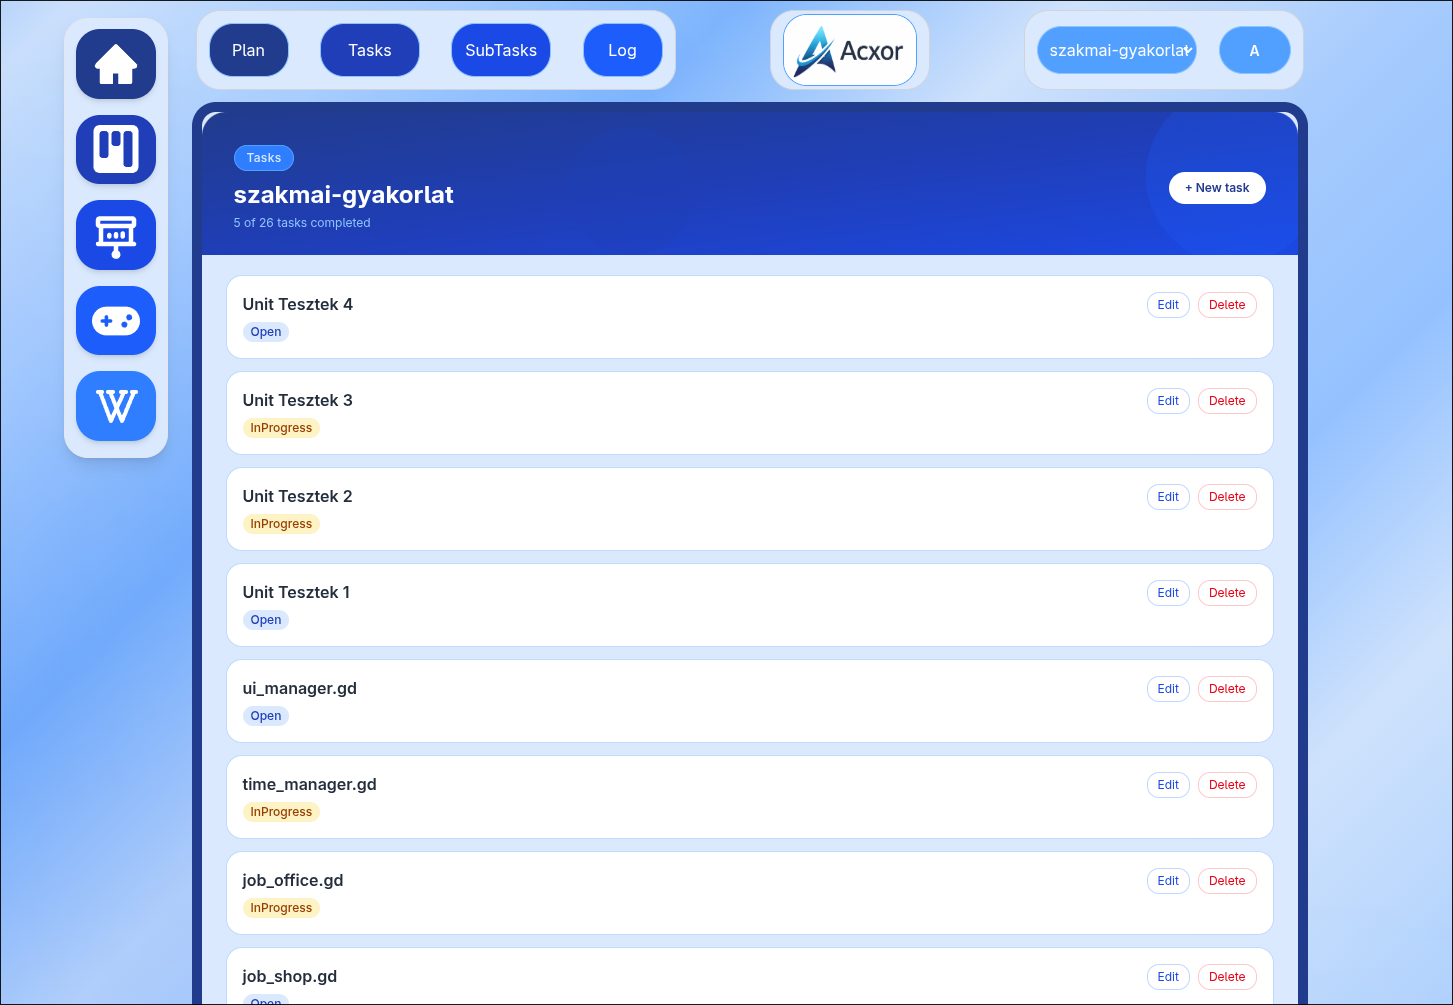
\includegraphics[width=0.8\textwidth]{images/frontend_tasks.png}
\caption{A TasksView komponens megjelenése}
\label{fig:architecture}
\end{figure}

\SubSection{Kanban nézet}

A \texttt{KanbanView} három oszlopban jeleníti meg a feladatokat (\texttt{Open}, \texttt{InProgress}, \texttt{Done}). Az oszlopok dinamikusan kiszámított adatokat kapnak: minden oszlop szűri a globális \texttt{tasks} tömbből a saját státuszához tartozó elemeket. Az oszlopok fejlécein megjelenik a benne lévő feladatok száma, az egyes kártyákon látható a felelős felhasználó és a határidő.

\begin{figure}[h!]
\centering
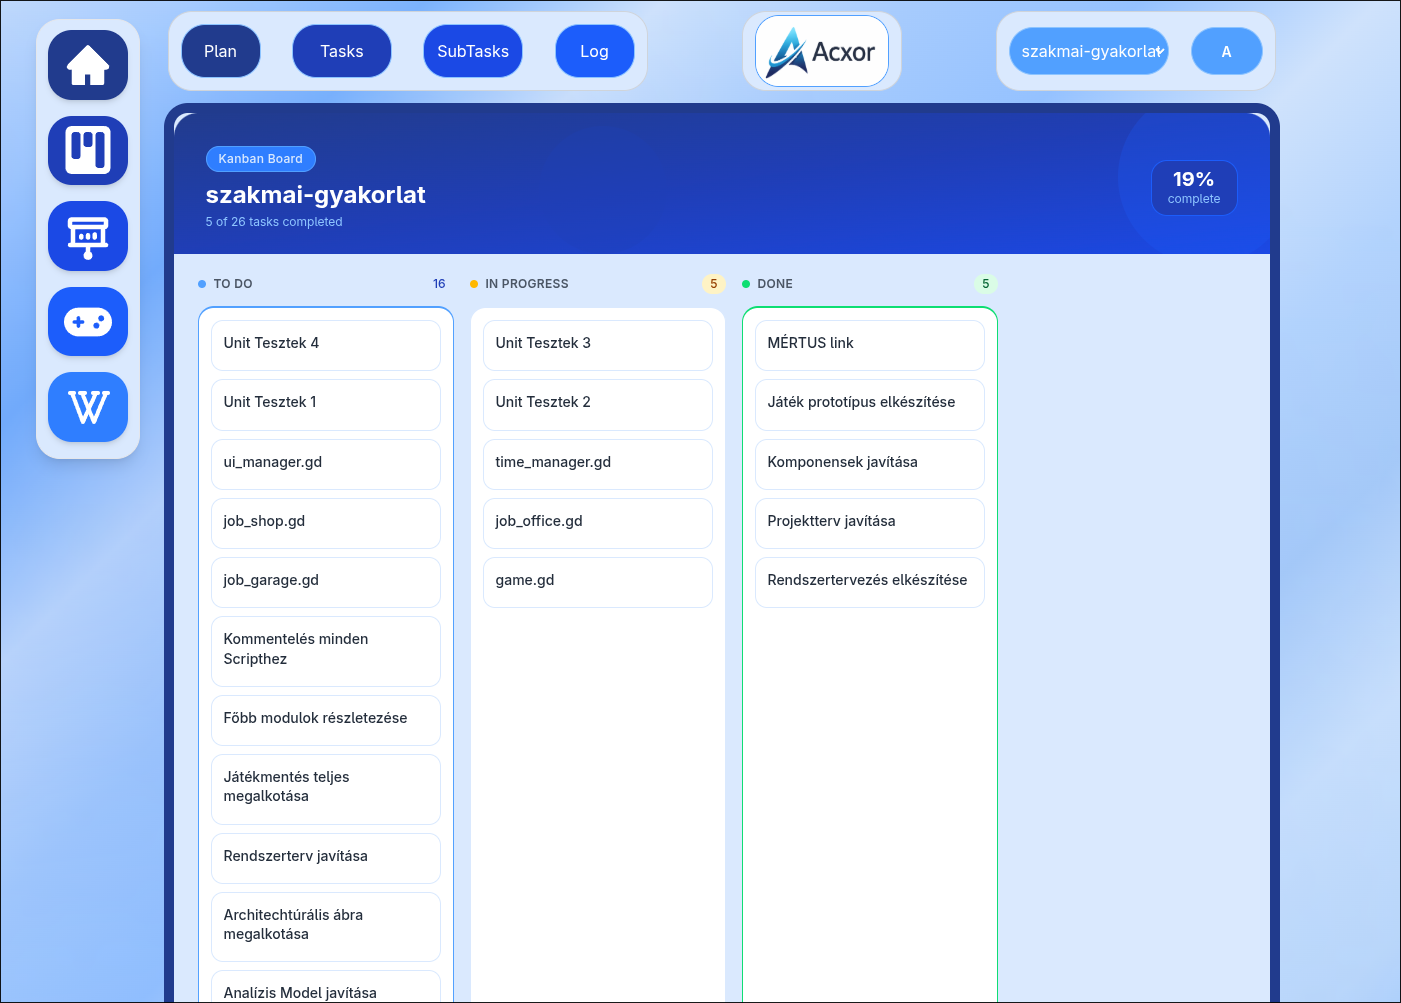
\includegraphics[width=0.8\textwidth]{images/frontend_kanban.png}
\caption{A KanbanView komponens megjelenése}
\label{fig:architecture}
\end{figure}

\SubSection{Scrum nézet}

A \texttt{ScrumView} a legösszetettebb nézetek egyike: egyszerre kezeli a sprint kiválasztást, sprint létrehozást, feladatok sprinthez rendelését, és a Kanban-szerű sprint boardot. A sprinthez nem rendelt feladatok a „Backlog" szekcióban jelennek meg. A sprint kiválasztó gombok tetején az aktív sprint (amelynek dátumtartománya lefedi az aktuális dátumot) egy zöld „active" badget kap. A sprint törlése után az érintett feladatok automatikusan visszakerülnek a backlogba (a backend kezeli ezt a konzisztenciát).

\begin{figure}[h!]
\centering
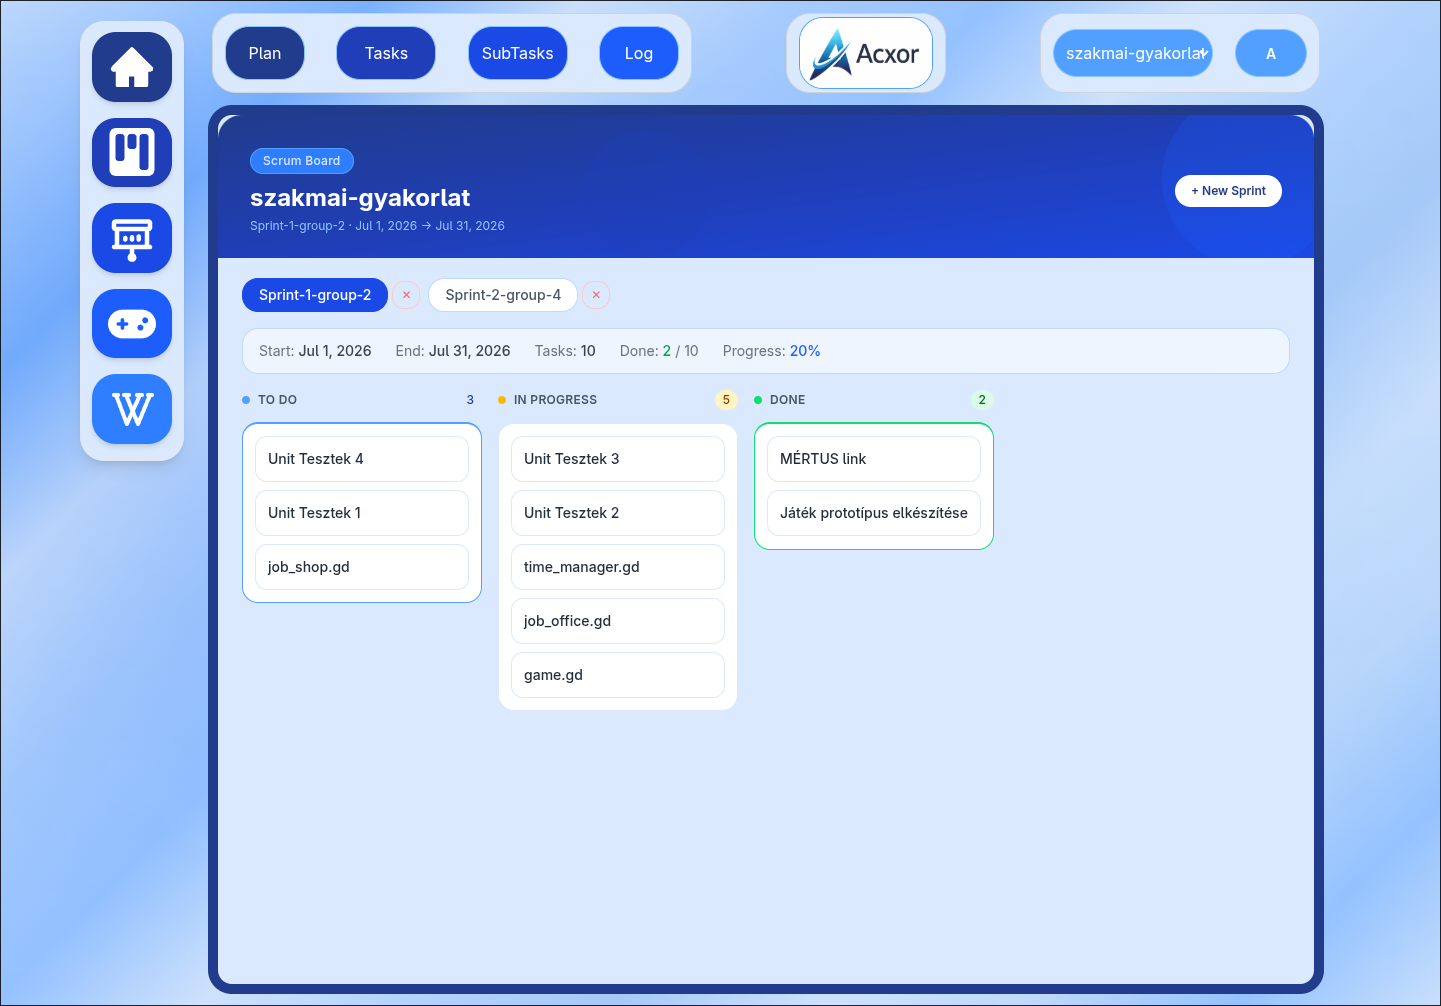
\includegraphics[width=0.8\textwidth]{images/frontend_scrum.png}
\caption{A ScrumView komponens megjelenése}
\label{fig:architecture}
\end{figure}

\SubSection{Gamifikáció nézet}

A \texttt{GamificationView} egy ranglistát jelenít meg a projekt tagjai számára. A felhasználókat XP és szint szerint rendezi, az első helyen lévő felhasználó kártyája arany szegéllyel kiemelve jelenik meg. Minden kártyán látható a felhasználó szintje, XP értéke, a következő szinthez szükséges XP, az XP progress bar és a megszerzett badge szintek. A gamifikációs rendszer magyarázatát egy kinyitható accordion panel tartalmazza, amelyben a szintlépési formula, a prestige rendszer és a class badge-ek kerülnek bemutatásra.

\begin{figure}[h!]
\centering
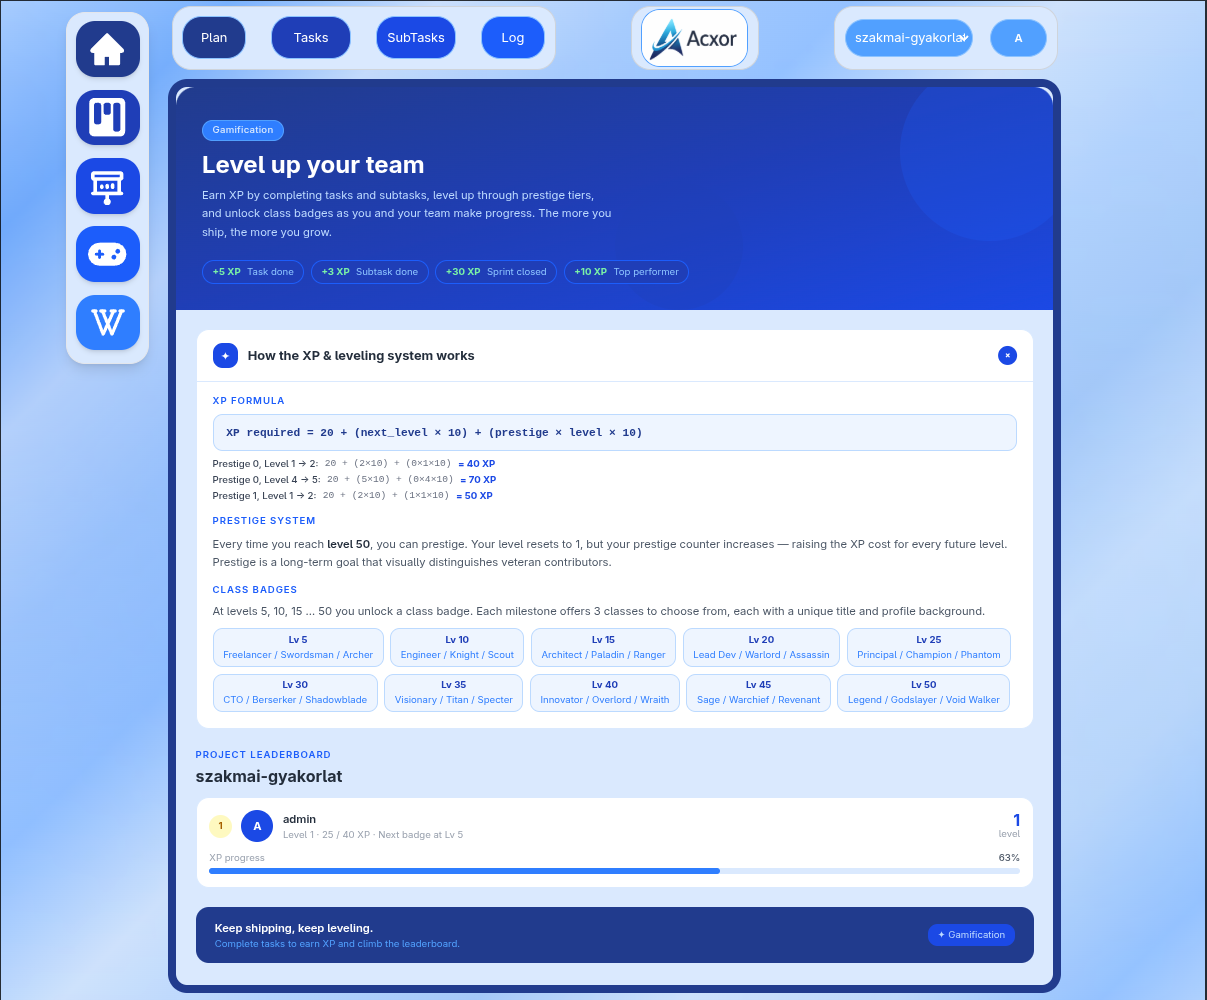
\includegraphics[width=0.8\textwidth]{images/frontend_game.png}
\caption{A GamificationView komponens megjelenése}
\label{fig:architecture}
\end{figure}

\SubSection{Mail rendszer}

A levelezési rendszer (\texttt{Mails} komponens) háromrészes elrendezést alkalmaz: egy hero fejléc, egy bal oldali levéllista panel (inbox / sent tab váltóval) és egy jobb oldali olvasó/szerkesztő panel. Az olvasási műveletnél a leveleket automatikusan olvasottnak jelöli a rendszer egy \texttt{PUT} kéréssel, és az olvasatlan levelek száma a hero fejlécben és az inbox tab feliratán is megjelenik. Az összeállítási nézet inline jelenik meg a jobb panelben, nem modálban.

% ─────────────────────────────────────────────────────────────────────────────
\Section{Mobil alkalmazás implementáció}
% ─────────────────────────────────────────────────────────────────────────────

\SubSection{Navigáció}

A mobil alkalmazás navigációja Expo Router segítségével valósul meg. A \texttt{(tabs)} csoportban tíz tab lap él: index (főoldal), tasks, subtasks, kanban, scrum, plan, gamification, mails, log, account. Az önálló képernyők (sign, create-project) a Stack navigátor részeként érhetők el. A tab bar egyedi komponensként lett megvalósítva (\texttt{CustomTabBar}), mivel az alapértelmezett Expo tab bar nem támogatta a vízszintes görgetést, amely tíz tab esetén szükségessé vált.

\begin{lstlisting}[language=JavaScript, caption={Egyedi tab bar implementáció (_layout.tsx)}]
function CustomTabBar({ state, navigation }) {
  return (
    <View style={styles.tabBarWrapper}>
      <ScrollView horizontal showsHorizontalScrollIndicator={false}>
        {TABS.map((tab, index) => {
          const focused = state.index === index;
          return (
            <TouchableOpacity
              key={tab.name}
              style={[styles.tabItem,
                      focused && styles.tabItemActive]}
              onPress={() => navigation.navigate(tab.name)}
            >
              {tab.icon(focused)}
              <Text style={[styles.tabLabel,
                            focused && styles.tabLabelActive]}>
                {tab.label}
              </Text>
            </TouchableOpacity>
          );
        })}
      </ScrollView>
    </View>
  );
}
\end{lstlisting}

\SubSection{Projekt választó}

Mivel a mobil alkalmazásban nincs topbar-szerű elem, a projektválasztás egy modal alapú \texttt{ProjectPicker} komponensen keresztül valósul meg. A komponens egy \texttt{TouchableOpacity} gombot jelenít meg az aktuális projekt nevével, és kattintásra egy alulról felcsúszó modal nyílik, amelyen az összes projekt listázva jelenik meg. A kiválasztott projekt azonnal frissíti a globális állapotot.

\SubSection{Alfeladatok nézet}

A mobil \texttt{SubtasksScreen} egy kinyitható/becsukható struktúrát alkalmaz: minden feladatkártya fejléce koppintható, és mutatja vagy elrejti az adott feladathoz tartozó alfeladatokat. Ez a döntés szükséges volt a mobilon elérhető kisebb képernyős terület miatt. Az alfeladatok hozzáadása inline szövegbeviteli mezőn keresztül, szerkesztésük pedig egy alulról felemelkedő modálban történik.

\SubSection{API kommunikáció}

A mobil alkalmazás a webes klienstől eltérően nem axio-st, hanem a beépített \texttt{fetch} API-t használja a HTTP kérésekhez. Ez tudatos döntés volt: csökkenti a függőségek számát, és a React Native fejlesztők által is preferált megoldás. Az API URL-t a \texttt{constants/api.ts} fájl konfigurálja dinamikusan: Expo Go fejlesztői módban a \texttt{Constants.expoConfig.hostUri} alapján automatikusan meghatározza a fejlesztői gép LAN IP-jét, így fizikai eszközön is működik a fejlesztés.

\begin{lstlisting}[language=JavaScript, caption={Dinamikus API URL (constants/api.ts)}]
const debuggerHost =
  Constants.expoConfig?.hostUri?.split(':')[0];

const BASE = debuggerHost
  ? `http://${debuggerHost}:5000/api`
  : 'http://localhost:5000/api';

export const API_URL = BASE;
\end{lstlisting}

\begin{figure}[h!]
\centering
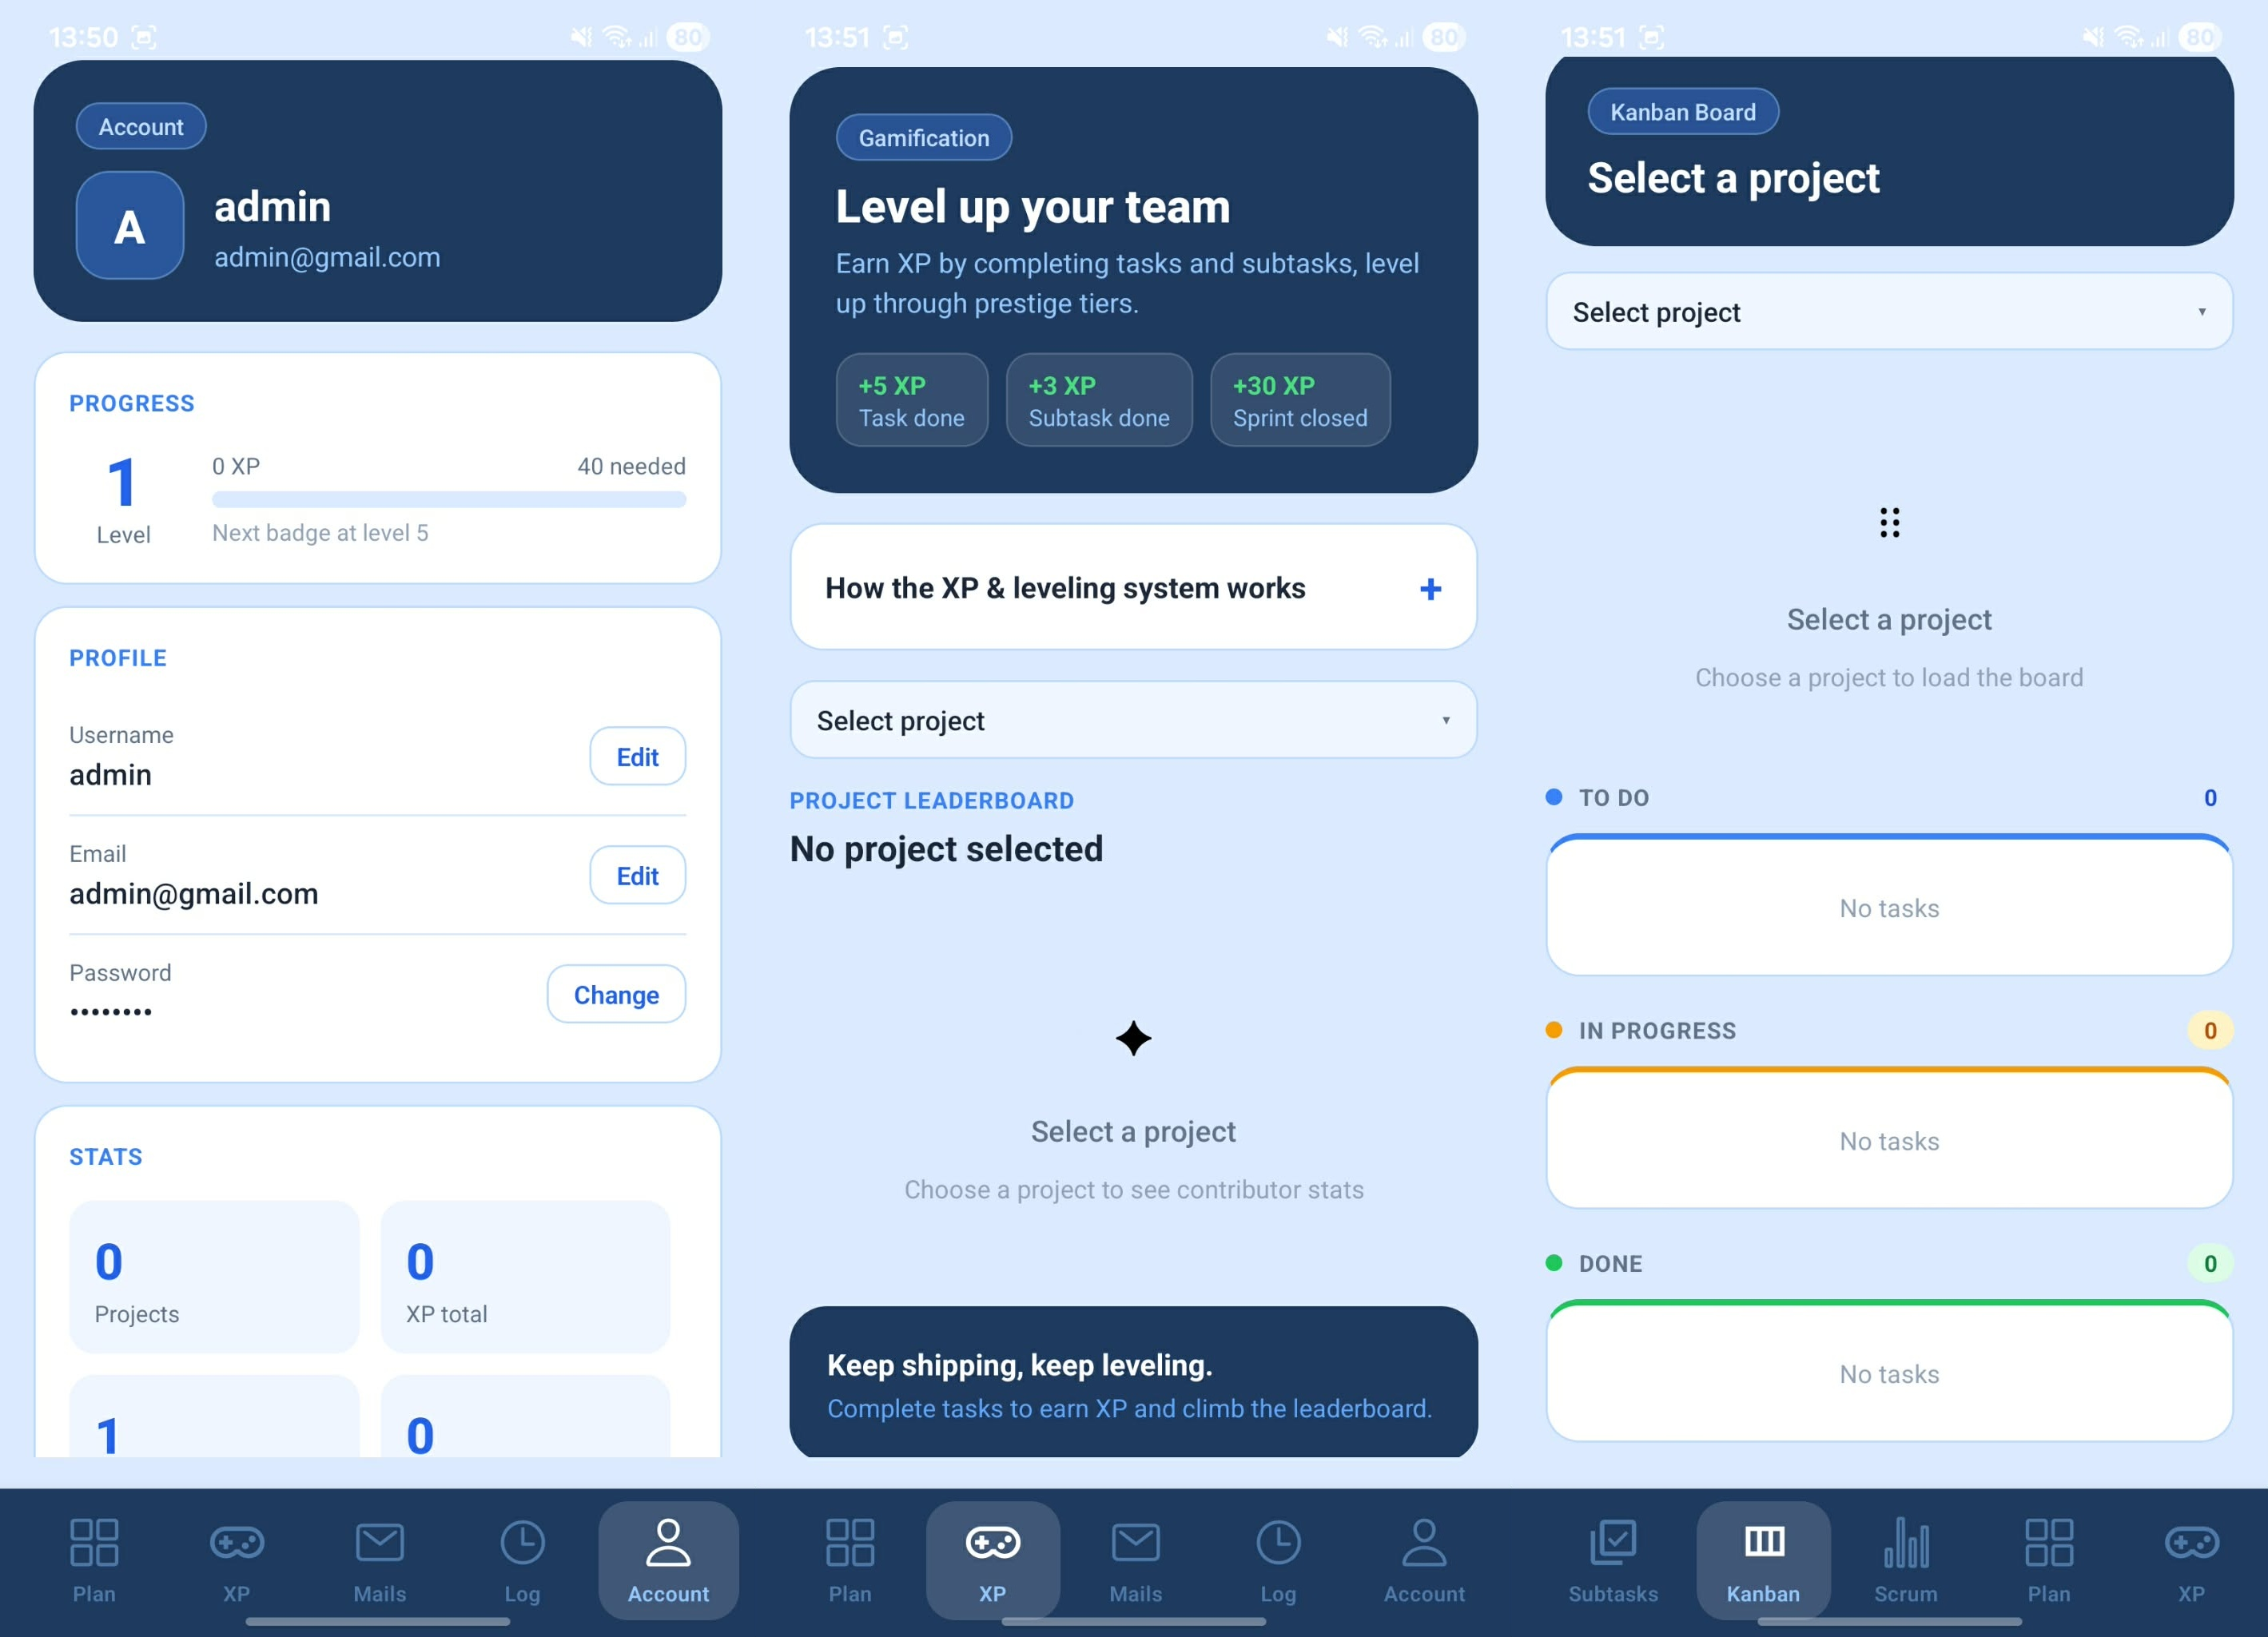
\includegraphics[width=0.8\textwidth]{images/mobile_screens.png}
\caption{A mobil alkalmazás főbb nézetei}
\label{fig:architecture}
\end{figure}

% ─────────────────────────────────────────────────────────────────────────────
\Section{Tesztelés implementációja}
% ─────────────────────────────────────────────────────────────────────────────

A rendszer tesztelése két szinten valósul meg: backend oldalon Jest és Supertest segítségével írt integrációs tesztek, frontend oldalon Vitest és React Testing Library alapú unit tesztek.

\SubSection{Backend tesztelés}

A backend tesztek in-memory MongoDB adatbázist alkalmaznak (\texttt{mongodb-memory-server}), ami azt jelenti, hogy a tesztek nem igényelnek élő adatbázis-kapcsolatot, és teljesen izoláltan futnak. A \texttt{setup.ts} fájl minden tesztfájl előtt elindítja a memóriaadatbázist, és minden egyes teszt után törli az összes kollekcióból az adatokat, hogy biztosítsa az izolált futtatást.

\begin{lstlisting}[language=JavaScript, caption={Teszt setup (\_\_tests\_\_/setup.ts)}]
beforeAll(async () => {
  mongoServer = await MongoMemoryServer.create();
  await mongoose.connect(mongoServer.getUri());
});

afterEach(async () => {
  const collections = mongoose.connection.collections;
  for (const key in collections)
    await collections[key].deleteMany({});
});

afterAll(async () => {
  await mongoose.disconnect();
  await mongoServer.stop();
});
\end{lstlisting}

Az integrációs tesztek a Supertest könyvtár segítségével közvetlenül az Express alkalmazásnak küldenek HTTP kéréseket, és ellenőrzik a visszakapott státuszkódot, a válasz testét és az adatbázis állapotát. A tesztek lefedik az auth, project, task, subtask és service szintű működést.

\begin{figure}[h!]
\centering
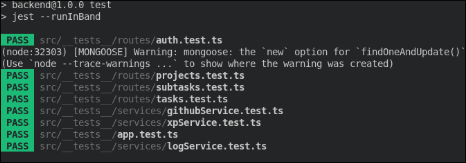
\includegraphics[width=0.8\textwidth]{images/jest_tests.png}
\caption{A backend tesztek futtatásának eredménye}
\label{fig:architecture}
\end{figure}

\SubSection{Frontend tesztelés}

A webes frontend tesztjei Vitest és React Testing Library segítségével készültek. A tesztek négy fő területet fednek le:

\begin{enumerate}
\item \textbf{Reducer tesztek}: Az \texttt{AppReducer} és \texttt{ViewReducer} függvények elszigetelt tesztelése, verifikálva, hogy minden action típus a várt állapotváltozást eredményezi.
\item \textbf{Context tesztek}: A \texttt{GlobalContext} és \texttt{ViewContext} tesztelése egyszerű tesztkomponenseken keresztül, ellenőrizve a dispatch-re adott re-render viselkedést.
\item \textbf{Action tesztek}: A \texttt{fetchTasks} és \texttt{addTask} action creator függvények tesztelése mockolt axios segítségével, verifikálva a helyes API hívást és dispatch sorozatot.
\item \textbf{Komponens tesztek}: A \texttt{Sign}, \texttt{CreateProject}, \texttt{TasksView} és \texttt{SubTasksView} komponensek renderelési és interakciós tesztjei, mockolt Context segítségével.
\end{enumerate}

\begin{lstlisting}[language=JavaScript, caption={TasksView unit teszt (Vitest)}]
it('rendereli a TasksView-t', () => {
  vi.spyOn(GlobalContext, 'useGlobalContext').mockReturnValue({
    state: {
      tasks: [
        { _id: '1', title: 'Task 1', status: 'open' },
        { _id: '2', title: 'Task 2', status: 'done' },
      ],
      selectedProject: { _id: 'proj1' },
      // ... egyéb mezők
    },
    dispatch: vi.fn(),
  });

  render(<TasksView />);
  expect(screen.getByText('Tasks')).toBeInTheDocument();
  expect(screen.getByText('Task 1')).toBeInTheDocument();
  expect(screen.getByText('Task 2')).toBeInTheDocument();
});
\end{lstlisting}

\begin{figure}[h!]
\centering
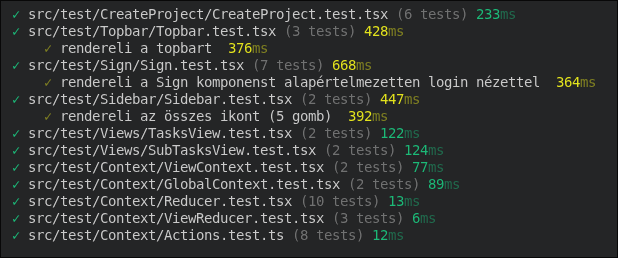
\includegraphics[width=0.8\textwidth]{images/vitest_tests.png}
\caption{A frontend tesztek futtatásának eredménye}
\label{fig:architecture}
\end{figure}

\SubSection{GitHub service tesztelés}

A \texttt{githubService.ts} tesztelése érdekes kihívást jelentett, mivel a GitHub API-t nem szerettük volna valóban hívni a tesztek során. Az axios mockolt verziójával (\texttt{jest.mock('axios')}) a tesztek ellenőrzik, hogy a service függvények a helyes URL-t hívják-e, a helyes headereket küldik-e el, és a válasz adatait a várt formátumra alakítják-e. A \texttt{logService.ts} tesztelésénél a \texttt{console.log} spy-olásával ellenőriztük, hogy a naplóbejegyzések a várt formátumban kerülnek kiírásra.

% ─────────────────────────────────────────────────────────────────────────────
\Section{Fejlesztési kihívások és megoldások}
% ─────────────────────────────────────────────────────────────────────────────

A fejlesztés során számos praktikus kihívással kellett szembenézni, amelyek megoldása tanulságos volt.

\textbf{Alfeladat betöltés párhuzamos kérésekkel}: Az alfeladatokat feladatonként kellett betölteni, ami azt jelentette, hogy ha egy projektnek 10 feladata van, 10 párhuzamos API kérés fut le. Ha a Redux-szerű \texttt{SET\_SUBTASKS} action-t használtuk volna, az egymást felülíró dispatch hívások miatt csak az utolsó kérés eredménye maradt volna meg. A megoldás az \texttt{APPEND\_SUBTASKS} action bevezetése volt, amely az adott feladathoz tartozó korábbi alfeladatokat kiszűri, majd az újakkal egészíti ki az állapotot.

\textbf{Mobil eszköz és localhost}: Fizikai mobileszközön a \texttt{localhost} nem mutat a fejlesztői gépre, hanem magára az eszközre. Az Expo által elérhető \texttt{Constants.expoConfig.hostUri} mező tartalmazza a fejlesztői szerver IP-jét és portját, amelyből a gép LAN IP-je kinyerhető. Ez az automatikus konfiguráció tette lehetővé, hogy a mobil app fejlesztés közben fizikai eszközön is futtatható legyen.

\textbf{Sprint törlés és feladat konzisztencia}: Sprint törlésekor a hozzá rendelt feladatokon is el kell végezni a sprint referencia törlését, különben azok sosem kerülnek vissza a backlogba. A backend sprint törlési route-ja azonban ezt nem oldja meg automatikusan – ez egy ismert hiányosság, amelyet az összefoglalóban is megemlítünk a jövőbeli fejlesztési irányok között.

\textbf{Swagger dokumentáció hiánya}: Bár a tervezési fejezetben Swagger UI képernyőkép szerepel, a fejlesztés során külső Swagger dokumentáció nem készült automatikusan. Az API végpontok dokumentálása kézzel, \texttt{swagger-jsdoc} vagy hasonló eszközzel utólag is elvégezhető lett volna – ez szintén egy jövőbeli fejlesztési lehetőség.
\Chapter{Tesztelés}

A tesztelési fejezet részletesen bemutatja az Acxor rendszer tesztelési stratégiáját, az alkalmazott eszközöket, a tesztesetek felépítését és az elért eredményeket. A tesztelés célja annak igazolása, hogy az implementált funkciók az elvárásoknak megfelelően működnek, és hogy a jövőbeli módosítások regressziót ne okozzanak a meglévő működésben.

% ─────────────────────────────────────────────────────────────────────────────
\Section{Tesztelési stratégia}
% ─────────────────────────────────────────────────────────────────────────────

A rendszer tesztelése két jól elkülönített rétegben valósult meg. A backend oldalon integrációs tesztek ellenőrzik a teljes kérés-válasz ciklust, beleértve az adatbázissal való interakciót, a hitelesítési logikát és az üzleti szabályok érvényesítését. A frontend oldalon egységtesztek verifikálják az állapotkezelési logikát, az action creator függvényeket és a legfontosabb UI komponensek helyes renderelését.

A tesztelési megközelítés a következő elveket követi:
\begin{itemize}
  \item Minden teszteset független és izolált: a tesztek között nincs közös állapot, az adatbázis tartalma minden teszteset után törlődik.
  \item A tesztek lehetőség szerint a rendszer külső viselkedését ellenőrzik, nem belső implementációs részleteket.
  \item A tesztek a fejlesztéssel párhuzamosan készültek, nem utólag.
  \item Ahol a külső rendszerek (GitHub API) nem hívhatók valódi tesztekben, mockolt adatokkal dolgozunk.
\end{itemize}

% ─────────────────────────────────────────────────────────────────────────────
\Section{Backend tesztelés}
% ─────────────────────────────────────────────────────────────────────────────

\SubSection{Eszközök és konfiguráció}

A backend tesztek Jest tesztelési keretrendszert és Supertest HTTP tesztkönyvtárat alkalmaznak. A Jest biztosítja a tesztfuttatót, az assertionokat és a mock funkcionalitást. A Supertest lehetővé teszi, hogy az Express alkalmazásnak valódi HTTP kéréseket küldjünk anélkül, hogy portot kellene foglalni, így a tesztek gyorsan és izoláltan futnak.

Az adatbázis szintű izoláció érdekében a \texttt{mongodb-memory-server} könyvtár egy in-memory MongoDB példányt indít el minden tesztfájl futtatásakor. Ez azt jelenti, hogy a tesztek semmilyen körülmények között nem érintik az éles vagy fejlesztési adatbázist. A \texttt{\_\_tests\_\_/setup.ts} fájl konfigurálja ezt a mechanizmust, és a Jest \texttt{globalSetup} vagy \texttt{setupFilesAfterEnv} konfigurációján keresztül kerül betöltésre.

\SubSection{Auth tesztek}

A hitelesítési tesztek a \texttt{POST /api/auth/register} és \texttt{POST /api/auth/login} végpontokat fedik le. A regisztrációs tesztek ellenőrzik:

\begin{itemize}
  \item Sikeres regisztráció esetén 201-es státuszkód és érvényes JWT token visszaadása.
  \item A jelszó nem jelenik meg a válaszban (adatbiztonság).
  \item Duplikált e-mail esetén 400-as hiba és megfelelő üzenet visszaadása.
  \item A visszaadott token érvényes JWT formátumú (három pontosvesszővel elválasztott Base64 szegmens).
  \item Az alapértelmezett XP és level értékek helyesek (\texttt{xp: 0}, \texttt{level: 1}).
\end{itemize}

A bejelentkezési tesztek ellenőrzik a helyes adatokkal való sikeres bejelentkezést, a helytelen jelszóra adott 400-as választ, a nem létező e-mailre adott hibaüzenetet, és azt, hogy bejelentkezés válaszában sem szerepel a jelszó.

\begin{lstlisting}[language=JavaScript, caption={Regisztrációs teszt részlet (auth.test.ts)}]
it('a jelszó nem kerül vissza a válaszban', async () => {
  const res = await request(app)
    .post('/api/auth/register')
    .send(validUser);

  expect(res.body.user).not.toHaveProperty('password');
});

it('a visszaadott token érvényes JWT formátumú', async () => {
  const res = await request(app)
    .post('/api/auth/register')
    .send(validUser);

  const jwtPattern =
    /^[A-Za-z0-9-_]+\.[A-Za-z0-9-_]+\.[A-Za-z0-9-_]+$/;
  expect(res.body.token).toMatch(jwtPattern);
});
\end{lstlisting}

\SubSection{Projekt tesztek}

A projekt tesztek a teljes CRUD ciklust lefedik. Minden teszteset saját felhasználót regisztrál (\texttt{registerAndLogin} segédfüggvény), így biztosítva az izolációt. A lefedett esetek:

\begin{itemize}
  \item Projekt létrehozása helyes adatokkal (201), token nélkül (401), hiányzó névvel (400).
  \item A létrehozó automatikusan adminisztrátor és tag lesz.
  \item TaskGroup-okkal való projektlétrehozáskor a feladatok és alfeladatok létrejönnek az adatbázisban.
  \item Érvénytelen tokennel való kísérlet 401-et ad vissza.
  \item A projektek listázása csak a saját projektek tartalmazza (más felhasználóé nem jelenik meg).
  \item Az admin mező populálva érkezik vissza (jelszó nélkül).
  \item Projekt módosítása és törlése csak az adminisztrátornak engedélyezett (másnak 403).
  \item Törléskor a kapcsolódó feladatok és alfeladatok is törlődnek.
\end{itemize}

\begin{lstlisting}[language=JavaScript, caption={Projekt törlési teszt (projects.test.ts)}]
it('törli a projektet és az összes kapcsolódó task-ot', async () => {
  const createRes = await request(app)
    .post('/api/projects')
    .set('Authorization', `Bearer ${token}`)
    .send({
      name: 'Törlendő projekt',
      taskGroups: [{
        name: 'Sprint 1', deadline: '2025-07-01',
        tasks: [{ description: 'Törlendő task',
                   subtasks: ['Sub 1'] }],
      }],
    });

  const projectId = createRes.body._id;

  const deleteRes = await request(app)
    .delete(`/api/projects/${projectId}`)
    .set('Authorization', `Bearer ${token}`);

  expect(deleteRes.status).toBe(200);

  const remainingTasks = await Task.find({ project: projectId });
  expect(remainingTasks).toHaveLength(0);
});
\end{lstlisting}

\SubSection{Feladat tesztek}

A task tesztek a feladatok létrehozását, lekérését, módosítását és törlését fedik le. Fontos tesztesetek:

\begin{itemize}
  \item A feladat alapértelmezett státusza \texttt{'Open'}.
  \item A határidő (\texttt{deadline}) helyesen tárolódik és visszaadódik.
  \item A státusz módosítható (pl. \texttt{'Open'} $\rightarrow$ \texttt{'InProgress'}).
  \item Törlés után a feladat nem jelenik meg a projekt feladatlistájában.
  \item Token nélküli hozzáférés 401-es hibát ad.
\end{itemize}

\SubSection{Alfeladat tesztek}

Az alfeladat tesztek hasonló struktúrát követnek, mint a feladattesztek, kiegészítve az XP alapértékének ellenőrzésével (\texttt{xpReward: 0}) és az XP mező módosíthatóságával.

\SubSection{Service tesztek}

\textbf{xpService tesztek}: Az \texttt{addXP} függvény tesztelése az in-memory adatbázison fut (nem mockolt), így valódi Mongoose dokumentumokon ellenőrizzük a viselkedést. A tesztesetek:

\begin{itemize}
  \item XP hozzáadásakor az érték helyesen növekszik.
  \item Küszöbérték elérésénél szintlépés következik be (maradék XP-vel).
  \item Több szintlépés egyszerre is működik.
  \item Nulla XP hozzáadása nem változtatja meg az állapotot.
  \item Nem létező felhasználóra hiba dobódik (\texttt{'User not found'}).
  \item A szint és XP az adatbázisban is perzisztálódik.
  \item Pontosan a küszöbön lévő XP szintlépést okoz, maradék 0 XP-vel.
\end{itemize}

\begin{lstlisting}[language=JavaScript, caption={XP szintlépési teszt (xpService.test.ts)}]
it('több szintet lép egyszerre, ha sok XP érkezik', async () => {
  const user = await createUser(0, 1);
  // 1. szint: 100 XP, 2. szint: 200 XP -> 300 XP kell a 3. szinthez
  const updated = await addXP(user._id.toString(), 350);

  expect(updated.level).toBe(3);
  expect(updated.xp).toBe(50);
});
\end{lstlisting}

\textbf{githubService tesztek}: Az axios modul teljes mocking-jával teszteljük, hogy a service a helyes GitHub API URL-eket hívja-e, a helyes Authorization headert küldi-e el, és a válasz adatait a várt formátumra alakítja-e (pl. \texttt{creator} mező a \texttt{user.login}-ból).

\textbf{logService tesztek}: A \texttt{console.log} spy-olásával ellenőrizzük, hogy a naplóbejegyzések a várt formátumban (\texttt{[PROJECT id] üzenet}) kerülnek kiírásra. Ez a teszt a log mentési logikát is verifikálja, de mivel a log service az adatbázisba is ír, a tesztek in-memory DB-n futnak.

% ─────────────────────────────────────────────────────────────────────────────
\Section{Frontend tesztelés}
% ─────────────────────────────────────────────────────────────────────────────

\SubSection{Eszközök és konfiguráció}

A frontend tesztek Vitest tesztelési keretrendszert és React Testing Library-t alkalmaznak. A Vitest Vite-alapú, és natívan kezeli a TypeScript-et és a JSX-et. A React Testing Library a komponensek felhasználói szemszögből való tesztelésére ösztönöz: nem az implementáció részleteit, hanem a látható és interakcióra képes elemeket ellenőrzi.

A tesztek konfigurációja a Vitest konfigurációs fájlban a \texttt{jsdom} tesztkörnyezetet alkalmazza, a \texttt{@testing-library/jest-dom} pedig bővíti a matchers listát (pl. \texttt{toBeInTheDocument}, \texttt{toHaveProperty}).

\SubSection{Reducer tesztek}

A reducer tesztek a legegyszerűbbek: tiszta függvényeket tesztelnek, amelyeknek nincs mellékhatásuk. Az \texttt{AppReducer} tesztjei ellenőrzik a \texttt{SET\_SUBTASKS}, \texttt{SET\_LOADING} és \texttt{SET\_SELECTED\_PROJECT} action típusokat. A \texttt{ViewReducer} tesztjei verifikálják az ismeretlen action típusra adott alapértelmezett viselkedést, és az összes \texttt{ViewState} értékkel való kompatibilitást.

\begin{lstlisting}[language=JavaScript, caption={ViewReducer tesztek (ViewReducer.test.tsx)}]
it('SET_VIEW akció frissíti az activeView-t', () => {
  const action: ViewAction = { type: 'SET_VIEW', payload: 'tasks' };
  const newState = ViewReducer(initialViewState, action);
  expect(newState).toBe('tasks');
});

it('többféle ViewState-et is kezel', () => {
  const states: ViewState[] =
    ['main', 'kanban', 'scrum', 'subtasks', 'log'];
  states.forEach((state) => {
    const newState = ViewReducer(initialViewState,
      { type: 'SET_VIEW', payload: state });
    expect(newState).toBe(state);
  });
});
\end{lstlisting}

\SubSection{Context tesztek}

A Context tesztek egyszerű tesztkomponenseket renderelnek a Context Providerbe ágyazva, és ellenőrzik az alapértelmezett állapotot, majd egy gombnyomás szimulációjával a dispatch utáni állapotváltozást.

\begin{lstlisting}[language=JavaScript, caption={GlobalContext integrációs teszt}]
it('dispatch frissíti a token-t és user-t', () => {
  render(
    <GlobalProvider>
      <TestComponent />
    </GlobalProvider>,
  );

  fireEvent.click(screen.getByText('Set User'));
  expect(screen.getByText('Token: abc123')).toBeInTheDocument();
});
\end{lstlisting}

\SubSection{Action tesztek}

Az action tesztek az axios mock-olásával ellenőrzik, hogy a \texttt{fetchTasks} és \texttt{addTask} függvények a helyes URL-t hívják-e, a megfelelő headereket küldik-e el, és a szerver válasza alapján a helyes dispatch hívásokat indítják-e el. Hibaeset szimulációjával ellenőrizzük a \texttt{SET\_ERROR} dispatch-t is.

\SubSection{Komponens tesztek}

\textbf{Sign komponens}: A tesztek ellenőrzik, hogy mindkét form (Register és Login) renderelésre kerül, a form submit az adatokkal meghívja a megfelelő action függvényt, és a loading / error állapotok megjelennek a felületen.

\textbf{CreateProject komponens}: A tesztek verifikálják a kezdő lépés megjelenítését, a Manual flow következő lépésre váltást, a contributor hozzáadás működését, és hogy üres contributor nem adható hozzá.

\textbf{TasksView és SubTasksView komponensek}: Mockolt globális állapottal ellenőrzik, hogy a feladatok és alfeladatok cím szerint megjelennek-e a nézetben.

\textbf{Sidebar és Topbar}: Strukturális tesztek ellenőrzik, hogy a megfelelő számú gomb és a várt HTML elem (\texttt{header} szerepkör) megjelenik-e.

\begin{table}[h!]
\centering
\small
\begin{tabularx}{\textwidth}{|l|Y|c|}
\hline
\textbf{Tesztkészlet} & \textbf{Lefedett esetek} & \textbf{Tesztek száma} \\
\hline
auth.test.ts & Regisztráció, bejelentkezés, token validáció & 9 \\
projects.test.ts & CRUD, jogosultság, taskGroup import & 11 \\
tasks.test.ts & CRUD, állapotváltás, határidő kezelés & 8 \\
subtasks.test.ts & CRUD, alapértékek, XP mező & 8 \\
xpService.test.ts & XP hozzáadás, szintlépés, perzisztencia & 8 \\
githubService.test.ts & API hívások, adat transzformáció & 11 \\
logService.test.ts & Naplóformátum, userId kezelés & 5 \\
app.test.ts & Alapvető route ellenőrzés & 1 \\
\hline
\textbf{Backend összesen} & & \textbf{61} \\
\hline
Reducer.test.tsx & AppReducer action típusok & 3 \\
ViewReducer.test.tsx & ViewReducer állapotváltás & 3 \\
GlobalContext.test.tsx & Context alapállapot, dispatch & 2 \\
ViewContext.test.tsx & View váltás dispatch-csel & 2 \\
Actions.test.ts & fetchTasks, addTask, hibakezelés & 3 \\
Sign.test.tsx & Form render, submit, loading/error & 4 \\
CreateProject.test.tsx & Lépések, contributor kezelés & 4 \\
TasksView.test.tsx & Feladatlista renderelés & 1 \\
SubTasksView.test.tsx & Alfeladatlista renderelés & 1 \\
Sidebar.test.tsx & Ikonok száma & 1 \\
Topbar.test.tsx & Banner elem & 1 \\
\hline
\textbf{Frontend összesen} & & \textbf{25} \\
\hline
\textbf{Összes teszteset} & & \textbf{86} \\
\hline
\end{tabularx}
\caption{A tesztkészletek összefoglalása}
\label{tab:test-summary}
\end{table}

% ─────────────────────────────────────────────────────────────────────────────
\Section{Manuális tesztelés}
% ─────────────────────────────────────────────────────────────────────────────

Az automatizált tesztek mellett a rendszer manuális tesztelésen is átesett. Ennek során a következő folyamatokat ellenőriztük végig a böngészőben és fizikai mobil eszközön:

\begin{itemize}
  \item Teljes regisztráció és bejelentkezés folyamata.
  \item Projekt létrehozása manuálisan és GitHub importtal.
  \item Feladatok és alfeladatok hozzáadása, szerkesztése, törlése és befejezése.
  \item XP jóváírás és szintlépés ellenőrzése a főoldalon és a gamification nézetben.
  \item Sprint létrehozása, feladat hozzárendelése és sprint törlése.
  \item Belső levelezés küldése és fogadása két különböző felhasználói fiókkal.
  \item Aktivitásnapló megjelenítésének ellenőrzése különböző műveletek elvégzése után.
  \item Profil szerkesztés (felhasználónév, e-mail, jelszó módosítás).
  \item Mobil alkalmazás teljes funkcionalitásának ellenőrzése Android eszközön (Expo Go).
\end{itemize}

\begin{figure}[h!]
\centering
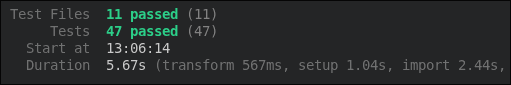
\includegraphics[width=0.8\textwidth]{images/vitest_results.png}
\caption{A frontend unit tesztek futtatásának eredménye (Vitest)}
\label{fig:architecture}
\end{figure}

\begin{figure}[h!]
\centering
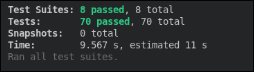
\includegraphics[width=0.8\textwidth]{images/jest_results.png}
\caption{A backend integrációs tesztek futtatásának eredménye (Jest)}
\label{fig:architecture}
\end{figure}

% ─────────────────────────────────────────────────────────────────────────────
\Section{Ismert korlátok és nem tesztelt területek}
% ─────────────────────────────────────────────────────────────────────────────

A tesztelés nem teljes körű, és számos terület kívül esett a tesztlefedettségen. A mail rendszer backend végpontjai nem kaptak dedikált integrációs teszteket, bár a modell és a route struktúrája megegyezik a többi, tesztelt erőforrással. A sprint feladat-hozzárendelési logika részletes edge case-jei (pl. egy feladat két sprinthez rendelése egymás után) szintén nem kerültek automatizált tesztekbe. A mobil alkalmazás frontend komponenseire nem készültek unit tesztek, elsősorban az Expo és React Native tesztkörnyezet konfigurálásának összetettsége miatt. A teljesítménytesztelés (load testing, stressz teszt) szintén nem volt a dolgozat keretein belül.

Ezek a hiányosságok tudatos döntések eredménye: az elérhető idő és erőforrás keretek között a legkritikusabb üzleti logika (auth, XP, project/task/subtask CRUD) kapta a legnagyobb tesztlefedettséget.
\Chapter{Összefoglalás}

% ─────────────────────────────────────────────────────────────────────────────
\Section{A munka összegzése}
% ─────────────────────────────────────────────────────────────────────────────

A dolgozat egy modern, háromplatformos projektmenedzsment rendszer, az Acxor teljes körű tervezését és implementációját mutatta be. A rendszer egy közös Node.js/Express backend API köré épül, amelyhez egy React alapú webes alkalmazás és egy React Native/Expo alapú mobil alkalmazás csatlakozik kliensként. Mindhárom platform TypeScript-ben íródott, ami egységes kódbázis-szemléletet és típusbiztonságot biztosít az egész rendszerben.

A bevezetőben megfogalmazott alapproblémára -- miszerint a meglévő projektmenedzsment eszközök vagy túlságosan komplexek, vagy túlságosan egyszerűek, és ritkán párosítják a professzionális funkcionalitást motivációs elemekkel -- az Acxor egy letisztult, vizuálisan koherens és gamifikációs elemekkel dúsított megoldást kínál. A koncepciós fejezetben elvégzett piackutatás alapján az Acxor a Trello vizuális egyszerűségét, a JIRA sprint-alapú munkaszervezési képességét és a rendszerek által általában elhanyagolt motivációs réteget ötvözi egyetlen platformban.

A tervezési fejezetben részletesen bemutatásra kerültek az architektúrális döntések: a háromrétegű kliens-szerver modell, a MongoDB adatbázis-séma és a hét Mongoose modell (User, Project, Task, Subtask, Sprint, Log, Mail), a RESTful API tervezési elvei és a JWT alapú hitelesítési folyamat. A felhasználói felület tervezésekor a hangsúly az egységes vizuális identitáson és a három platform közötti konzisztens élményen volt. Külön figyelmet kapott a karbantarthatóság kérdése: a közös állapotkezelési minta, az API contract szerepe és a tudatosan vállalt kódduplikáció mint kezelt technikai adósság mind a tervezési döntések szerves részét képezték.

Az implementációs fejezetben a legfontosabb megvalósítási részletek kerültek terítékre: a backend route-ok és service-ek, az XP és szintlépési algoritmus, a Context API alapú állapotkezelés, a nézetek és komponensek felépítése, valamint a GitHub integrációs megoldás. A mobil alkalmazásnál külön figyelmet kapott az egyedi tab bar megoldás és a fizikai eszközön való fejlesztést lehetővé tevő dinamikus API URL konfiguráció.

A tesztelési fejezetben összesen 86 teszteset kerül bemutatásra: 61 backend integrációs teszt (Jest + Supertest + mongodb-memory-server) és 25 frontend unit teszt (Vitest + React Testing Library). A tesztek lefedik a hitelesítési logikát, a projekt és feladat CRUD műveleteket, az XP service szintlépési algoritmusát, a GitHub service adat-transzformációját és a legfontosabb React komponensek renderelési viselkedését.

% ─────────────────────────────────────────────────────────────────────────────
\Section{Elért eredmények}
% ─────────────────────────────────────────────────────────────────────────────

A fejlesztés során az alábbi főbb eredmények születtek:

\begin{itemize}
  \item \textbf{Teljes körű REST API}: Kilenc végpontcsoport (auth, projects, tasks, subtasks, sprints, logs, users, mails, github) mindegyike authentikált hozzáférést biztosít, és következetesen kezeli a hibákat.
  \item \textbf{Gamifikációs rendszer}: A befejezett feladatokért és alfeladatokért XP jár, amelynek mértéke szintlépéskor csökkenti a fennmaradó értéket, és automatikusan növeli a szintet. A prestige rendszer tovább mélyíti a hosszú távú motivációt.
  \item \textbf{Webes alkalmazás}: Kanban board, Scrum sprint kezelés, Plan nézet projekt-szintű statisztikákkal, alfeladat kezelés, aktivitásnapló, belső levelezési rendszer, gamifikáció rangsor, wiki és fiókkezelés -- mind egyetlen oldalas, Context API alapú alkalmazásban.
  \item \textbf{Mobil alkalmazás}: Az összes fő funkció elérhető Expo Router alapú, tíz tapos navigációval rendelkező React Native alkalmazásban, fizikai Android és iOS eszközön egyaránt.
  \item \textbf{GitHub integráció}: Repozitóriumok listázása és issue-k importálása feladatokként, szerver oldalon proxyzva a GitHub API-n keresztül.
  \item \textbf{Tesztlefedettség}: 86 automatizált teszteset, amelyek a rendszer kritikus üzleti logikáját és API viselkedését verifikálják.
  \item \textbf{Karbantartható architektúra}: Egységes állapotkezelési minta a webes és mobil kliensben, service réteg szétválasztása a route handlerektől, TypeScript típusbiztonság mindhárom platformon, és közös backend mint egyetlen igazságforrás a két kliens számára.
\end{itemize}

% ─────────────────────────────────────────────────────────────────────────────
\Section{A karbantarthatóság értékelése}
% ─────────────────────────────────────────────────────────────────────────────

A rendszer fejlesztése során a karbantarthatóság nem utólagos szempont volt, hanem tervezési alapelv. Ennek értékelése három dimenzióban végezhető el: a kódbázis struktúrája, a web–mobil összehangoltság és a jövőbeli bővíthetőség szempontjából.

\SubSection{Kódbázis struktúrájának karbantarthatósága}

A backend kódja jól elkülönített rétegekre épül: a route handlerek kizárólag a HTTP kérések fogadásáért és a válasz küldéséért felelősek, az üzleti logika a service rétegben él (\texttt{xpService}, \texttt{logService}, \texttt{githubService}), az adathozzáférés pedig a Mongoose modelleken keresztül valósul meg. Ez a háromrétegű szétválasztás azt jelenti, hogy például az XP számítási logika megváltoztatásához egyetlen fájlt (\texttt{xpService.ts}) kell módosítani, és az összes érintett végpont automatikusan az új logikát alkalmazza. Az ilyen jellegű, jól lokalizálható módosíthatóság a karbantartható szoftverek egyik legfontosabb jellemzője.

A TypeScript használata mindhárom platformon szintén közvetlen karbantarthatósági előnyt jelent: a típusrendszer fordítási időben jelzi az inkompatibilis változásokat, amelyek dinamikusan típusos kódban csak futásidőben derülnének ki. Ez különösen értékes akkor, amikor az adatmodell változik, és a változásnak mindhárom platformon át kell propagálódnia.

\SubSection{Web és mobil kliens összehangoltsága}

A webes React alkalmazás és a React Native mobil alkalmazás közötti karbantarthatóság legfőbb biztosítéka a közös állapotkezelési minta. Mindkét kliens ugyanolyan struktúrájú Context-et, Reducer-t és action creator függvényeket alkalmaz, ami azt jelenti, hogy egy fejlesztő, aki az egyik kliensben eligazodik, minimális tanulással képes a másikban is hatékonyan dolgozni. A közös backend API pedig garantálja, hogy az adatmodell változásai mindkét klienshez egyszerre jutnak el, és nem lehetséges, hogy a két kliens eltérő adatszerkezettel dolgozzon.

Ugyanakkor a dolgozat őszintén elismeri a jelenlegi architektúra korlátait is. Az \texttt{Actions.ts} fájlban lévő aszinkron action creator logika, a TypeScript interfész definíciók és a hibakezelési konvenciók mindkét kliensben kézzel vannak karbantartva, ami azt jelenti, hogy egy üzleti logika változásakor két helyen kell elvégezni az azonos módosítást. Ez a duplikáció kontrollált és tudatosan vállalt, de hosszú távon -- különösen csapatnövekedés esetén -- érdemes lenne megszüntetni egy megosztott csomag (shared package) bevezetésével.

\SubSection{Összegző értékelés}

Összességében az Acxor architektúrája a karbantarthatóság szempontjából egyensúlyt tart a pragmatizmus és az elvek között. A rendszer nem törekszik a tökéletes kódduplikáció-mentességre, ha az azzal járó komplexitás nem arányos az előnyökkel – de minden fontosabb architekturális döntés mögött felismerhető a karbantarthatósági szempont: a service réteg szétválasztása, a közös állapotkezelési minta, a TypeScript típusbiztonság és a tesztlefedettség együtt olyan rendszert alkotnak, amelyen egy új fejlesztő a belépéstől kezdve hatékonyan tud dolgozni, és amelyen a változtatások hatása előre látható és kontrollálható.

% ─────────────────────────────────────────────────────────────────────────────
\Section{Jövőbeli fejlesztési lehetőségek}
% ─────────────────────────────────────────────────────────────────────────────

A rendszer számos irányban tovább fejleszthető. A legfontosabb jövőbeli lehetőségek az alábbiak:

\textbf{Monorepo és megosztott csomag}: A karbantarthatóság legjelentősebb javítása egy monorepo struktúra (pl. Nx vagy Turborepo) bevezetése lenne, amelyen belül egy \texttt{shared} csomag tartalmazná a TypeScript interfész definíciókat, az action típusokat és a közös üzleti logikát. Ez megszüntetné a jelenlegi kódduplikációt a webes és mobil kliens között, és garantálná, hogy az adatmodell változásai automatikusan és konzisztensen érvényre jutnak mindkét kliensben -- jelentősen csökkentve az összehangolási hibák kockázatát.

\textbf{API contract és típusgenerálás}: A backend TypeScript interfészeit jelenleg kézzel másolják a kliensek. Egy OpenAPI/Swagger séma alapú típusgenerálási pipeline (pl. \texttt{openapi-typescript} eszközzel) lehetővé tenné, hogy a backend interfészei automatikusan generált típusként legyenek elérhetők mindkét kliensben. Ez az API contract szinkronizálási problémát teljesen megszüntetné: ha a backend változik, a következő generálási lépés után a kliensek azonnal látják a típusinkompatibilitást.

\textbf{Drag-and-drop a Kanban boardon}: A jelenlegi implementáció statikus kártyákat jelenít meg. A feladatok húzással való áthelyezése oszlopok között -- és ezzel egyidejűleg az állapot módosítása -- jelentősen javítaná a felhasználói élményt. Ez webes oldalon például a \texttt{@dnd-kit} könyvtárral valósítható meg.

\textbf{Valós idejű frissítések}: A jelenlegi rendszer lekérdezés alapú: az adatok akkor frissülnek, ha a felhasználó navigál vagy manuálisan frissít. WebSocket vagy Server-Sent Events alapú megoldással (pl. Socket.io) a csapat tagjai valós időben láthatnák egymás változtatásait.

\textbf{E-mail értesítések}: Feladat hozzárendeléskor vagy határidő közeledésekor automatikus e-mail értesítés küldése (pl. Nodemailer és egy SMTP szolgáltató segítségével).

\textbf{Sprint törlés és feladat konzisztencia}: Jelenleg sprint törlésekor a hozzá rendelt feladatok \texttt{sprint} mezője nem törlődik automatikusan a backendben, ami konzisztencia-problémát okozhat. Ezt egy MongoDB aggregációs pipeline-nal vagy Mongoose middleware-rel lehetne kezelni.

\textbf{Szerepkör-alapú jogosultságkezelés}: A jelenlegi rendszer megkülönböztet adminisztrátor és közreműködő szerepköröket, de a végrehajtási logika nem minden végponton érvényes egységesen. Egy részletesebb middleware-alapú permission réteg pontosabb hozzáférésvezérlést biztosítana.

\textbf{Prestige és class badge rendszer teljes kiépítése}: A gamifikációs tervezés tartalmaz egy class badge rendszert (szintenként három osztály közül lehet választani), amelynek UI-ja elkészült, de a mögötte lévő adatmodell (választott osztály tárolása) még nem implementált.

\textbf{Tesztlefedettség bővítése}: A mail rendszer backend integrációs tesztjei, a sprint tesztek és a mobil alkalmazás komponens tesztjei mind hasznos kiegészítések lennének a jövőbeli fejlesztések során. A mobil tesztelés hiánya elsősorban az Expo tesztkörnyezet konfigurálásának összetettsége miatt maradt el, de egy \texttt{jest-expo} alapú konfiguráció ezt orvosolhatná.

\textbf{Swagger/OpenAPI dokumentáció}: Az API végpontok automatikus dokumentálása swagger-jsdoc vagy tsoa segítségével interaktív, böngészhető dokumentációt biztosítana a jövőbeli integrációs partnerek és fejlesztők számára.

% ─────────────────────────────────────────────────────────────────────────────
\Section{Zárszó}
% ─────────────────────────────────────────────────────────────────────────────

Az Acxor fejlesztése megmutatta, hogy egy közepes komplexitású, háromplatformos alkalmazás megtervezése és implementálása egyetlen fejlesztőként is megvalósítható, ha a technológiai döntések jól vannak meghozva és a kódstruktúra kezdettől fogva gondosan ki van alakítva. A közös backend API, az újrafelhasznált üzleti logika és a konzisztens állapotkezelési minta lehetővé tette, hogy a három platform -- webes, mobil és szerver -- szorosan összehangoltan működjön.

A karbantarthatóság szempontjából a projekt egyik legfontosabb tanulsága az, hogy a webes és mobil kliens közötti konzisztencia nem jön magától: tudatos tervezési döntéseket igényel, amelyeket már az architektúra kialakításakor meg kell hozni. A közös állapotkezelési minta és a közös backend API mint egyetlen igazságforrás megfelelő alapot adott ehhez, ugyanakkor a kódduplikáció és az API contract manuális szinkronizálásának kérdése rámutat arra, hogy egy megosztott csomag alapú megközelítés a rendszer következő fejlődési lépése lehet.

A dolgozat elkészítése során személyes fejlődés is tapasztalható volt: a TypeScript alkalmazása kikényszerítette a pontosabb gondolkodást az adatstruktúrák körül, az automatizált tesztelés megkövetelte a moduláris kódszervezést, a mobil fejlesztés pedig új kihívásokat hozott a navigáció, a natív UI komponensek és a fizikai eszközön való fejlesztés terén.

Az Acxor jelenlegi formájában egy funkcionális, tesztelt és bővíthető alapot jelent. A jövőbeli fejlesztési lehetőségek gazdag tárháza nyitva áll, és a rendszer architektúrája -- különösen a service réteg szétválasztása, a TypeScript típusbiztonság és az egységes állapotkezelési minta -- ezeket a bővítményeket lehetővé teszi anélkül, hogy az alap kódbázist drasztikusan át kellene alakítani.

\clearpage

\addcontentsline{toc}{chapter}{Irodalomjegyzék}
\bibliographystyle{plain}
\bibliography{dolgozat.bib}

\newpage

\pagestyle{empty}

\noindent \textbf{\Large Adathordozó használati útmutató}

\vskip 1cm

Az adathordozón a \textit{bsc-degree-project} nevű projekt forráskódja és dokumentációja található, amely három fő részből áll: egy Node.js/Express alapú backend, egy React alapú webes frontend, valamint egy Expo alapú mobilalkalmazás.

\vskip 0.5cm

\noindent \textbf{Az adathordozó tartalma:}

\begin{itemize}
    \item \texttt{dolgozat.pdf} -- a szakdolgozat végleges változata,
    \item \texttt{latex/} -- a dolgozat \LaTeX{} forráskódja,
    \item \texttt{backend/} -- a szerveroldali alkalmazás forráskódja (Node.js, Express, TypeScript, MongoDB),
    \item \texttt{frontend/} -- a webes felhasználói felület forráskódja (React, Vite, TypeScript, Tailwind CSS),
    \item \texttt{mobile/} -- a mobilalkalmazás forráskódja (React Native, Expo),
    \item \texttt{README.md} -- telepítési és használati útmutató.
\end{itemize}

\vskip 0.5cm

\noindent \textbf{Szükséges szoftverek telepítése:}

Az alábbi szoftvereket globálisan kell telepíteni a rendszerre a projekt futtatása előtt.

\vskip 0.3cm

\noindent \textit{1. Node.js (18-as vagy újabb verzió)}

\noindent Letölthető: \texttt{https://nodejs.org}

\noindent Telepítés ellenőrzése:
\begin{verbatim}
node -v
npm -v
\end{verbatim}

\noindent \textit{2. MongoDB Community Edition}

\noindent Letölthető: \texttt{https://www.mongodb.com/try/download/community}

\noindent Telepítés után az adatbázis-szerver indítása:
\begin{verbatim}
mongod --dbpath /data/db
\end{verbatim}

\noindent A MongoDB alapértelmezetten a \texttt{mongodb://localhost:27017} címen fut.

\vskip 0.3cm

\noindent \textit{3. Expo Go (opcionális, fizikai eszközön való teszteléshez)}

\noindent Telepíthető az iOS App Store-ból vagy a Google Play áruházból. A mobilalkalmazás indítása után a terminálban megjelenő QR-kódot kell beolvasni.

\vskip 0.5cm

\noindent \textbf{Telepítés és indítás:}

A függőségek telepítése a projekt gyökérkönyvtárából egyetlen paranccsal elvégezhető:

\begin{verbatim}
npm run setup
\end{verbatim}

Ha újratelepítés szükséges (például verziókonfliktus esetén):

\begin{verbatim}
npm run reset
npm run setup
\end{verbatim}

Ezt követően az egyes komponensek az alábbi sorrendben indítandók el, mindegyik külön terminálablakban:

\begin{enumerate}
    \item A MongoDB szerver elindítása: \texttt{mongod}
    \item A backend szerver: \texttt{cd backend \&\& npm run dev} \hfill (port: \texttt{5000})
    \item A webes frontend: \texttt{cd frontend \&\& npm run dev} \hfill (port: \texttt{5173})
    \item A mobilalkalmazás: \texttt{cd mobile \&\& npx expo start}
\end{enumerate}

A backend működéséhez szükséges egy \texttt{backend/.env} konfigurációs fájl, amely az alábbi változókat tartalmazza:

\begin{verbatim}
PORT=5000
MONGO_URI=mongodb://localhost:27017/<adatbázisnév>
JWT_SECRET=<titkos_kulcs>
\end{verbatim}

\end{document}